%TEX TS-program = xelatex
%!TEX encoding = UTF-8 Unicode
% Original Doc by Dr. Karin Sumongkayothin
% Last updated by Dr. Jidapa Kraisangka
%============ Logs ===========================
% % May 2, 2019 -- Dr. Karin Sumongkayothin
% [+] Figure caption centering was fixed
% [+] thesisGradyear variable was added
% [+] Landscape style was added
%---------------------------------------------
% June 1, 2019 -- Dr. Karin Sumongkayothin
% [+] Listing cation was set to aligned left
% [+] Remove using /raggedright in table captions
% [+] Correct the spaces between  Name and Lastname
% [+] Add title to student name in abstract page
%---------------------------------------------
% Aug 1, 2020 -- Dr. Jidapa Kraisangka
% [+] Fixed space between title and name for long first name
% [+] Clean some texts and provide example LaTex
%---------------------------------------------
% Sep 15, 2021 -- Dr. Jidapa Kraisangka
% [-] Remove DoB and Place of Birth from Biographies
%---------------------------------------------
%=============================================

\documentclass[16pt, a4paper]{book}
% \documentclass{report}
% \usepackage{fontspec}
\newcommand{\thesisCoadvTH}{}
\usepackage{ifthen}
\usepackage{graphicx}

\usepackage{fontspec}
\usepackage{xunicode}
\usepackage{xltxtra}


%====== Add the packages here ================
\usepackage{enumitem}
\setlist[itemize]{topsep=0.35\baselineskip,itemsep=0.15\baselineskip,parsep=0pt,partopsep=0pt,leftmargin=1.5em}
\usepackage{listings}	%For showing programming language in Latex
\usepackage{caption}
\usepackage{subcaption}
\captionsetup{compatibility=false}
\usepackage{xcolor}
\usepackage{amssymb}
\usepackage{pifont}

\newcommand{\cmark}{\ding{51}}
\newcommand{\xmark}{\ding{55}}

\usepackage{amsmath}
\usepackage[hidelinks]{hyperref}
\urlstyle{same}
\renewcommand{\UrlFont}{\normalfont}
\usepackage[section]{placeins}
\usepackage{booktabs}

\usepackage{textcomp}
\usepackage{multirow}
\usepackage{float}
\usepackage{lscape}
\usepackage{pdflscape}
% https://www.overleaf.com/project/5dc7fb1fd24fcd000117ca19

\usepackage{longtable}
\usepackage{array}

%update Mar 31 2023
\usepackage{adjustbox}
%=============================================

\makeatletter
\def\input@path{{styles/}}
\makeatother
\usepackage{muictthesis}
\newcolumntype{P}[1]{>{\raggedright\arraybackslash}p{#1}}
\usepackage{tabularx}

%%%%%%%%%%%%%%%%%%%%%%%%%%%%%%%%%%%%%%
%Set listing options
%%%%%%%%%%%%%%%%%%%%%%%%%%%%%%%%%%%%%%

\lstset{
columns=fullflexible,
float=h,
frame=single,
basicstyle=\fontsize{10}{10}\selectfont\ttfamily,
breaklines=true,
postbreak=\mbox{\textcolor{red}{$\hookrightarrow$}\space},
belowcaptionskip=8pt
}



%%%%%%%%%%%%%%%%%%%%%%%%%%%%%%%%%%%%%%
%Set path directory of figures
%%%%%%%%%%%%%%%%%%%%%%%%%%%%%%%%%%%%%%

%% Include more path to figures here
% \graphicspath{{./figures/chap1/}{./figures/chap2/}{./figures/chap3/}{./figures/chap4/}{./figures/chap5/}}

\XeTeXlinebreaklocale "th"	%Set word wrapping for Thai language
\XeTeXlinebreakskip = 0pt plus 1.1pt   %

%%%%%%%%%%%%%%%%%%%%%%%%%%%%%%%%%%%%%%
%Thesis Meta Data (edit each field)
%%%%%%%%%%%%%%%%%%%%%%%%%%%%%%%%%%%%%%
%Thesis Title
\newcommand{\thesisTitle}{Green code smell detection with Visual studio code extension}
\newcommand{\thesisTitleTH}{PyGreenSense: ระบบตรวจจับ Green Code Smell สำหรับภาษา Python บน VS Code}

% Thesis Keywords
\newcommand{\thesisKeywords}
{กรีนโค้ดสเมลล์ (GREEN CODE SMELL) \slash ภาษาไพธอน (PYTHON) \slash วิศวกรรมซอฟต์แวร์ที่ยั่งยืน (GREEN SOFTWARE ENGINEERING) \slash แอ็บสแตรกซินแทกซ์ทรี (AST) \slash SOFTWARE CARBON INTENSITY (SCI) \slash COSMIC FUNCTION POINT (CFP)}

%Author name
\newcommand{\thesisFirstTitleName}{Mr.}
\newcommand{\thesisFirstAuthorName}{Jittakan}
\newcommand{\thesisFirstAuthorLastName}{Damrongtrakoonwat}
\newcommand{\thesisFirstTitleNameTH}{นาย}
\newcommand{\thesisFirstAuthorNameTH}{จิตรกัณฐ์}
\newcommand{\thesisFirstAuthorLastNameTH}{ดำรงตระกูลวัฒน์}
\newcommand{\thesisFirstAuthorID}{6587051}
\newcommand{\thesisFirstAuthorBP}{Bangkok, Thailand}
\newcommand{\thesisFirstAuthorHC}{Bachelor of Science in Digital Science and Technology, Mahidol University, 2025}

\newcommand{\thesisSecondTitleName}{Mr.}		%Comment all if you don't have second author
\newcommand{\thesisSecondAuthorName}{Tutchakorn}
\newcommand{\thesisSecondAuthorLastName}{Gomonkongyou}
\newcommand{\thesisSecondTitleNameTH}{นาย}
\newcommand{\thesisSecondAuthorNameTH}{ธัชกร}
\newcommand{\thesisSecondAuthorLastNameTH}{โกมลคงอยู่}
\newcommand{\thesisSecondAuthorID}{6587055}
\newcommand{\thesisSecondAuthorBP}{Bangkok, Thailand}
\newcommand{\thesisSecondAuthorHC}{Bachelor of Science in Digital Science and Technology, Mahidol University, 2025}


\newcommand{\thesisThirdTitleName}{Mr.}			%Comment all if you don't have third author
\newcommand{\thesisThirdAuthorName}{Suntipap}
\newcommand{\thesisThirdAuthorLastName}{Chotimanont}
\newcommand{\thesisThirdTitleNameTH}{นาย}
\newcommand{\thesisThirdAuthorNameTH}{สันติภาพ}
\newcommand{\thesisThirdAuthorLastNameTH}{โชติมานนท์}
\newcommand{\thesisThirdAuthorID}{6587105}
\newcommand{\thesisThirdAuthorBP}{Yasothon, Thailand}
\newcommand{\thesisThirdAuthorHC}{Bachelor of Science in Digital Science and Technology, Mahidol University, 2025}

\newcommand{\thesisAuthorsInitials}{I1. Lastname1, I2.  Lastname2, I3. Lastname3} %Initials of Thesis Authors

%Degree that this thesis is for
\newcommand{\thesisDegree}{วิทยาศาสตรบัณฑิต}
\newcommand{\thesissubDegree}{สาขาวิทยาการและเทคโนโลยีดิจิทัล}

%Month, year and date of thesis publication
\newcommand{\thesisAcademicYear}{2025} %Academic Year
\newcommand{\thesisGradYear}{2025} %Graduated Year

%Department
%\newcommand{\thesisDep}{Faculty of Information and Communication Technology}
\newcommand{\thesisDep}{คณะเทคโนโลยีสารสนเทศและการสื่อสาร}

%University
%\newcommand{\thesisUni}{Mahidol University}
\newcommand{\thesisUni}{มหาวิทยาลัยมหิดล}

%Advisor name
\newcommand{\thesisAdv}{Assistant Professor Dr. Thanwadee Sunetnanta}		    %with title name
\newcommand{\thesisAdvTH}{ผู้ช่วยศาสตราจารย์ ดร. ธันวดี สุเนตนันท์}  		%with title name

%Co-advisor name
% \def\thesisCoadv{Dr. XXXXXX XXXXXXX}	%with title name; comment if you don't have co-advisor
% \def\thesisCoadvTH{ดร.xxxxx xxxxx}
%===========================================================
% Copyright
%\documentclass{article}
%\usepackage[printwatermark]{xwatermark}
%\usepackage{lipsum}


% \newwatermark*[allpages,color=red!50,angle=45,scale=3,xpos=0,ypos=0]{Copyright of Mahidol University}

\begin{document}
    \renewcommand{\thelstlisting}{\thechapter.\arabic{lstlisting}} %Change listing numbering style
    \makeatletter
    \makeatother
    \newpage
    \coverpage
    \begin{acknowledgement}

โครงงานเรื่อง PyGreenSense: ระบบตรวจจับ Green Code Smell สำหรับภาษา Python บน VS Code สำเร็จลุล่วงได้ด้วยความกรุณาและการสนับสนุนอย่างดียิ่งจาก ผู้ช่วยศาสตราจารย์ ดร. ธันวดี สุเนตนันท์ อาจารย์ที่ปรึกษาโครงงาน ผู้ซึ่งได้ให้คำแนะนำ ข้อคิดเห็น และตรวจสอบแก้ไขข้อบกพร่องต่าง ๆ มาโดยตลอดทุกขั้นตอนของการดำเนินโครงงาน คณะผู้จัดทำขอกราบขอบพระคุณเป็นอย่างสูงไว้ ณ โอกาสนี้

ท้ายที่สุดนี้ คณะผู้จัดทำหวังเป็นอย่างยิ่งว่าโครงงานฉบับนี้จะเป็นประโยชน์ต่อผู้ที่สนใจด้านการพัฒนาซอฟต์แวร์อย่างยั่งยืน การตรวจจับ Green Code Smell และการประยุกต์ใช้เครื่องมือวิเคราะห์โค้ดสำหรับภาษา Python เพื่อส่งเสริมการตระหนักรู้ด้านประสิทธิภาพพลังงานและผลกระทบต่อสิ่งแวดล้อมในการพัฒนาซอฟต์แวร์ต่อไป

\end{acknowledgement}


    \begin{abstractTH}

อุตสาหกรรมซอฟต์แวร์ที่เติบโตอย่างรวดเร็วส่งผลให้เกิดความต้องการทรัพยากรประมวลผลมหาศาล ซึ่งเป็นปัจจัยหนึ่งที่ก่อให้เกิดภาวะโลกร้อน โดยสาเหตุส่วนหนึ่งมาจากรูปแบบการเขียนโค้ดที่สิ้นเปลืองพลังงาน หรือการสร้างสิ่งที่เรียกง่า "Green Code Smells" ในโค้ด โครงงานนี้จึงพัฒนา "PyGreenSense" ซึ่งเป็นไลบรารีและส่วนขยายบน Visual Studio Code สำหรับตรวจจับ Green Code Smells ในภาษา Python เพื่อสร้างความตระหนักรู้เกี่ยวกับการเขียนโค้ดตามหลักการของวิศวกรรมซอฟต์แวร์ที่เป็นมิตรต่อสิ่งแวดล้อม (Green Software Engineering) แก่โปรแกรมเมอร์ที่สนใจผลกระทบในการเขียนโค้ดที่สิ้นเปลืองพลังงาน

ในโครงการนี้ ผู้พัฒนาได้ประยุกต์ใช้เทคนิค Abstract Syntax Tree (AST) เพื่อวิเคราะห์และระบุตำแหน่งโครงสร้างโค้ดที่สิ้นเปลืองทรัพยากร 5 ประเภท ได้แก่ God Class, Duplicated Code, Long Method, Mutable Default Arguments และ Dead Code พร้อมแสดงรายงานข้อผิดพลาดและประเมินการปล่อยคาร์บอนผ่านเครื่องมือ CodeCarbon นอกจากนี้ ยังผนวกตัวชี้วัดผลกระทบของคาร์บอนจากการกำจัด code smell เพื่อประเมินผลสัมฤทธิ์จากการปรับปรุงโค้ด ควบคู่กับการวัด Software Carbon Intensity (SCI) ต่อหน่วยฟังก์ชัน (SCI per CFP) ตามมาตรฐาน COSMIC Function Point (CFP) การทำงานเหล่านี้ช่วยให้โปรแกรมเมอร์สามารถประเมินการใช้พลังงานเทียบกับขนาดฟังก์ชันงาน และสร้างความตระหนักรู้ถึงความสัมพันธ์ระหว่างการเขียนโค้ดกับการใช้พลังงานได้อย่างเป็นรูปธรรม

\end{abstractTH}
    \newpage

    % \pagenumbering{gobble} % Remove page number from bottom
    %update 30 Mar 2023
    \fancyhead[r]{\thepage}
    \fancyfoot{}

    \tableofcontents
    \newpage

    %\lstlistoflistings
    \addtocontents{toc}{\vspace*{0.7\baselineskip}}%

    \mainmatter		%Reset and set page number to arabic style
    \renewcommand{\chaptermark}[1]{\markboth{#1}{}}
    \fancyhead[L]{\ifthenelse{\isodd{\value{page}}}{คณะ ICT มหาวิทยาลัยมหิดล}{}} %odd page header
    \fancyhead[R]{\ifthenelse{\isodd{\value{page}}}{ว.ทบ. (DST)~/~\thepage}{\leftmark~/~\thepage}} %even page header

    \chapter{บทนำ}
\label{Ch:Introduction}
ในปัจจุบัน ปัญหาการเปลี่ยนแปลงภูมิอากาศโลก เป็นประเด็นสำคัญที่ส่งผลกระทบทั้งต่อระบบนิเวศของสิ่งมีชีวิตและต่อระบบเศรษฐกิจ ซึ่งมีผลโดยตรงต่อคุณภาพชีวิตของผู้คนทั่วโลก ประเด็นดังกล่าวได้ก่อให้เกิดความตระหนักรู้และการร่วมมือกันในการปกป้อง พิทักษ์ และรักษาทรัพยากรธรรมชาติให้ยั่งยืน ในภาคส่วนซอฟต์แวร์และเทคโนโลยีสารสนเทศก็มีบทบาทสำคัญ เนื่องจากการพัฒนาซอฟต์แวร์ที่ไม่มีประสิทธิภาพอาจนำไปสู่การใช้พลังงานที่สูงเกินความจำเป็น ดังนั้นผู้จัดทำจึงมุ่งเน้นที่จะศึกษาและพัฒนา แนวทางการเขียนโปรแกรมเชิง Green Coding ผ่านภาษาคอมพิวเตอร์ที่ได้รับความนิยมอย่าง Python เพื่อเสนอเครื่อง
มือที่สามารถช่วยวิเคราะห์ผลกระทบต่อสิ่งแวดล้อมได้

ในบทนี้จะอธิบายถึงที่มาและความสำคัญของปัญหา วัตถุประสงค์ ขอบเขตการดำเนินงาน และประโยชน์ที่คาดว่าจะได้รับจากการศึกษาและพัฒนาเครื่องมือนี้

% -----------------------------------------------------

\section{ที่มาและความสำคัญของปัญหา}
\label{Sec:ProblemStatement}
ในปัจจุบันอุตสาหกรรมซอฟต์แวร์มีอัตราการเติบโตอย่างต่อเนื่อง ส่งผลให้ความต้องการใช้พลังงานสำหรับการประมวลผลเพิ่มสูงขึ้นตามไปด้วย การใช้พลังงานดังกล่าวยังส่งผลต่อทรัพยากรที่มีอยู่จำกัด ส่งผลกระทบต่อสิ่งแวดล้อมและการเปลี่ยนแปลงสภาพภูมิอากาศด้วยเช่นกัน

ผู้จัดทำเล็งเห็นถึงปัญหาการใช้พลังงานที่มากกว่าที่ควรซึ่งเกิดจากการพัฒนาซอฟต์แวร์ที่ไม่คำนึงถึงผลกระทบต่อการใช้พลังงาน จึงมุ่งเน้นการศึกษาการทำงานของ Green Code Smell เพื่อเป็นเครื่องมือช่วยตรวจสอบการทำงานของโค้ดในภาษา Python โดยจัดทำผลลัพธ์ในรูปแบบ Console Log, JSON และการแสดงผลเชิงภาพ (Visualization) ที่จะสะท้อนถึงประสิทธิภาพด้านการใช้พลังพลังงานและผลกระทบต่อสิ่งแวดล้อม อันจะนำไปสู่การส่งเสริมการพัฒนาซอฟต์แวร์ที่เป็นมิตรต่อสิ่งแวดล้อมมากยิ่งขึ้น

% -----------------------------------------------------

\section{วัตถุประสงค์}
\label{Sec:Objective}
โครงการนี้มีวัตถุประสงค์เพื่อสนับสนุนการพัฒนาซอฟต์แวร์อย่างยั่งยืน โดยมุ่งเน้นการตรวจจับและทำความเข้าใจรูปแบบโค้ดที่ส่งผลต่อการใช้พลังงาน (Green Code Smells) ในภาษา Python ผ่านการดำเนินการดังต่อไปนี้
\begin{enumerate}
    \item {\boldfont พัฒนาไลบรารีภาษา Python และส่วนขยายสำหรับ Visual Studio Code} \\
    เพื่อใช้ในการตรวจจับ Green Code Smells และรูปแบบการเขียนโปรแกรมอื่น ๆ ที่อาจส่งผลกระทบอย่างมีนัยสำคัญต่อการใช้พลังงานของซอฟต์แวร์ โดยรองรับการวิเคราะห์โค้ดอัตโนมัติและการประเมินเชิงโครงสร้าง
    \item {\boldfont ศึกษาผลกระทบด้านพลังงานของ Green Code Smells และพัฒนาวิธีการตรวจจับที่มีประสิทธิภาพ} \\
    โดยมุ่งเน้นการวิเคราะห์และทำความเข้าใจความสัมพันธ์ระหว่างรูปแบบโค้ดกับปริมาณการใช้พลังงาน รวมถึงการพัฒนา หรือการตรวจสอบความถูกต้องของวิธีการวิเคราะห์ที่ใช้ในการตรวจจับรูปแบบดังกล่าว
    \item {\boldfont สรุปผลและจัดทำข้อเสนอแนะเพื่อสนับสนุนการพัฒนาซอฟต์แวร์ที่ยั่งยืน} \\
    ผ่านการจัดทำรายงาน การแสดงผลผลการวิเคราะห์ และการประยุกต์ใช้ตัวชี้วัดด้านความยั่งยืนและการใช้พลังงาน เพื่อสนับสนุนให้ผู้พัฒนาสามารถปรับปรุงคุณภาพโค้ดตามแนวทาง Green Coding ได้อย่างมีประสิทธิภาพ
\end{enumerate}

% -----------------------------------------------------

\section{ขอบเขตงาน}
\label{Sec:ScopeOfWork}
โครงการนี้กำหนดขอบเขตการดำเนินงานเพื่อรองรับการพัฒนาและประเมินผล Green Code Smell Detector สำหรับภาษา Python โดยครอบคลุมประเด็นสำคัญดังต่อไปนี้
\begin{enumerate}
    \item {\boldfont การพัฒนาไลบรารีภาษา Python และส่วนขยายสำหรับ Visual Studio Code} \\
    พัฒนาไลบรารีและส่วนขยายเพื่อรองรับการตรวจสอบ Green Code Smells โดยใช้งานในเครื่องมือสำหรับการพัฒนาซอฟต์แวร์ที่มีความเป็นสากลอย่างเช่น Visual Studio Code
    \item {\boldfont รองรับการวิเคราะห์โค้ดด้วยโครงสร้าง Abstract Syntax Tree (AST)} \\
    ไลบรารีต้องสามารถประมวลผลและแยกวิเคราะห์โค้ดผ่านโครงสร้าง AST เพื่อสกัดองค์ประกอบของโค้ด เช่น Node, Statement และ Structure ต่าง ๆ เพื่อใช้ในการตรวจจับรูปแบบโค้ดที่ไม่ประหยัดพลังงาน
    \item {\boldfont ชุดของกฎเกณฑ์และการตรวจจับ Green Code Smell} \\
    กำหนดชุดของกฎเกณฑ์ (Ruleset) ตรรกะการสำหรับการวิเคราะห์ และเงื่อนไขเบื้องต้นสำหรับการตรวจจับ Green Code Smells โดยให้สอดคล้องกับแนวคิดเชิงโครงสร้างของภาษา Python และข้อมูลจากงานวิจัยที่เกี่ยวข้อง
    \item {\boldfont การประเมินและสรุปผลการวิเคราะห์โค้ด} \\
    ทำการสรุปผลการตรวจสอบโค้ด พร้อมจัดทำรายงานที่แสดงตัวชี้วัดที่สำคัญ เช่น การปล่อยคาร์บอน (Carbon Emission) การใช้พลังงาน (Energy Consumption) และตัวชี้วัดด้านความยั่งยืนอื่น ๆ เพื่อสนับสนุนการประเมินคุณภาพของโค้ด
\end{enumerate}

% -----------------------------------------------------

\section{ประโยชน์ที่คาดว่าจะได้รับ}
\label{Sec:ExpectedBenefit}
จากการดำเนินโครงการ มีความคาดหวังว่าจะได้ไลบรารี ที่สามารถใช้ตรวจสอบและวิเคราะห์ Green Code Smell ในภาษา Python ได้อย่างเป็นระบบ ซึ่งจะช่วยให้ผู้พัฒนาซอฟต์แวร์มีความตระหนักถึงผลกระทบต่อพลังงานและสิ่งแวดล้อมจากการเขียนโปรแกรม นอกจากนี้ยังสามารถใช้เป็นแนวทางเริ่มต้นในการประยุกต์แนวคิด Green Coding กับซอฟต์แวร์ประเภทอื่นในอนาคต โดยส่งเสริมการลดการใช้พลังงานที่ไม่จำเป็นและสนับสนุนการพัฒนาซอฟต์แวร์ที่ยั่งยืนและเป็นมิตรต่อสิ่งแวดล้อม

% -----------------------------------------------------

    \clearpage

    \chapter{ทฤษฎีที่เกี่ยวข้อง}
\label{Ch:Background}
การศึกษานี้ตั้งอยู่บนพื้นฐานของแนวคิดด้านพลังงานของซอฟต์แวร์ (Software Energy Consumption) แนวคิดด้าน Green Software Engineering และงานวิจัยหลายชิ้นที่สำรวจผลกระทบของ Design Patterns, Code Smells และ Refactoring ต่อประสิทธิภาพด้านพลังงานของระบบ เพื่อพัฒนาไลบรารีสำหรับตรวจจับ Green Code Smell ในภาษา Python อย่างเป็นระบบ งานวิจัยที่เกี่ยวข้องสามารถสรุปได้ดังนี้

% -----------------------------------------------------

\section{Green Software Engineering และพลังงานของซอฟต์แวร์}
งานสำรวจเชิงระบบโดย Poy et al.~\cite{poy2025impact} แสดงให้เห็นว่าการเลือกใช้ design patterns, การเกิด code smells และการ refactoring มีความสัมพันธ์โดยตรงกับการใช้พลังงานของซอฟต์แวร์ โดยพบว่าบาง design patterns สามารถช่วยลดการใช้พลังงานได้ในขณะที่บาง patterns อาจเพิ่มพลังงานขึ้นหากใช้งานไม่เหมาะสมซึ่งชี้ให้เห็นถึงความสำคัญของการออกแบบโค้ดให้มีความยั่งยืนตั้งแต่ต้นทาง

นอกจากนี้ Le Goaër~\cite{leGoaer2024tactics} ได้เสนอแนวคิด Green Tactics, Green Patterns และ Green Smells เพื่อใช้เป็นหลักการในการลดการทำงานที่สิ้นเปลืองทรัพยากรและเป็นรากฐานสำคัญของแนวทาง Green Code Smell Detection ในงานนี้

% -----------------------------------------------------

\section{Code Smells และผลกระทบด้านพลังงาน}
งานของ Verdecchia et al.~\cite{verdecchia2018energy} ถือเป็นหลักฐานเชิงประจักษ์สำคัญที่แสดงว่าการ refactor code smells สามารถลดการใช้พลังงานได้อย่างมีนัยสำคัญ โดยเฉพาะ code smells ประเภท Feature Envy และ Long Method ซึ่งเมื่อนำไป refactor แล้วให้ผลลัพธ์ลดการใช้พลังงานได้มากถึง 49.9\% ผลลัพธ์ดังกล่าวสนับสนุนสมมติฐานว่าการปรับโครงสร้างโค้ด สามารถส่งผลโดยตรงต่อพฤติกรรมด้านพลังงานของโปรแกรม

อย่างไรก็ตาม งานวิจัยดังกล่าวยังชี้ให้เห็นว่าไม่ใช่ทุก code smell ที่ให้ผลด้านพลังงานในทิศทางเดียวกันเช่น การ refactor God Class อาจเพิ่มจำนวนข้อความส่งระหว่างออบเจกต์ นำไปสู่การใช้พลังงานเพิ่มขึ้นแสดงให้เห็นถึงความซับซ้อนของความสัมพันธ์ระหว่าง “คุณภาพโค้ด” และ “ประสิทธิภาพด้านพลังงาน”

% -----------------------------------------------------

\section{Green Code Smells และ ecoCode}
ระบบ ecoCode ของ Le Goaër~\cite{legoaer2023ecocode} ได้ขยายความสามารถของ SonarQube เพื่อรองรับการตรวจจับ \textit{Green Code Smells} ซึ่งถูกนิยามว่าเป็น “รูปแบบการเขียนโค้ดที่ส่งผลต่อการใช้พลังงานหรือเพิ่ม Carbon Footprint ของซอฟต์แวร์” เครื่องมือนี้เน้นการตรวจจับปัญหาที่เกี่ยวข้องกับการใช้ API, ทรัพยากรฮาร์ดแวร์ และรูปแบบการประมวลผลที่ไม่เหมาะสมซึ่งถือเป็นฐานข้อมูลสำคัญในการประยุกต์ใช้กับภาษา Python ในงานนี้

เวอร์ชันที่ถูกเก็บใน HAL Archive~\cite{legoaer2023hal} ยังได้อธิบายโครงสร้างของ Green Code Smell Catalogue ซึ่งเป็นชุดกฎที่ไม่ได้ผูกติดกับภาษาใดภาษาเดียว แต่เน้นการวิเคราะห์โครงสร้างโค้ดในเชิงสถิติและพฤติกรรมการใช้พลังงาน ด้วยเหตุนี้ แนวคิดของ ecoCode จึงถูกนำมาใช้เป็นแม่แบบสำหรับการออกแบบกฎตรวจจับ Green Code Smell ของโปรเจกต์นี้

% -----------------------------------------------------

\section{มาตรวัดและการประเมินผลประสิทธิภาพการปล่อยคาร์บอน (Metrics and Evaluation)}
การประเมินความยั่งยืนของซอฟต์แวร์จำเป็นต้องมีดัชนีชี้วัดที่ชัดเจน เพื่อเปลี่ยนจากแนวคิดเชิงคุณภาพให้เป็นเชิงปริมาณ โดยมาตรฐานและแนวคิดที่สำคัญที่เกี่ยวข้องกับโครงงานนี้มีดังต่อไปนี้

\subsection{ข้อกำหนด Software Carbon Intensity (SCI)}
{\boldfont Software Carbon Intensity (SCI)} เป็นมาตรฐานที่นำเสนอโดย Green Software Foundation เพื่อใช้ในการคำนวณอัตราการปล่อยก๊าซเรือนกระจกของซอฟต์แวร์ต่อหนึ่งหน่วยการทำงาน (Functional Unit) โดยดัชนี SCI เน้นที่ ``ความเข้มข้น'' ของการปล่อยคาร์บอน และสามารถนำเสนอได้ในรูปของสมการต่อไปนี้~\cite{sciSpecification}

\[
SCI = \frac{(E \times I) + M}{R}
\]

คำอธิบายตัวแปรมีดังนี้
\begin{itemize}
    \item {\boldfont $E$ (Energy)}: พลังงานไฟฟ้าที่ซอฟต์แวร์ใช้ หน่วยเป็น kilowatt-hours (kWh)
    \item {\boldfont $I$ (Location-based Marginal Carbon Intensity)}: ค่าความเข้มข้นของคาร์บอนในสายส่งไฟฟ้า ณ เวลาและสถานที่นั้น ๆ หน่วยเป็น $gCO_2e/kWh$
    \item {\boldfont $M$ (Embodied Emissions)}: คาร์บอนที่เกิดขึ้นจากการผลิตและการจัดการวงจรชีวิตของฮาร์ดแวร์
    \item {\boldfont $R$ (Functional Unit)}: หน่วยวัดการทำงานของซอฟต์แวร์ เช่น ต่อจำนวนผู้ใช้งาน (User), ต่อการเรียกใช้ API (API Call) หรือต่อระยะเวลา (Time)
\end{itemize}

แนวคิดของ SCI มีความสำคัญต่อโครงงานนี้ เนื่องจากช่วยให้การประเมินผลด้านความยั่งยืนของซอฟต์แวร์ไม่หยุดอยู่เพียงการวัดพลังงานที่ใช้ทั้งหมด แต่สามารถเปรียบเทียบการปล่อยคาร์บอนต่อผลลัพธ์ของการทำงานได้อย่างเป็นระบบและเป็นธรรมมากขึ้น

\subsection{แนวคิดและวิธีการของ CodeCarbon}
CodeCarbon เป็นไลบรารีประเภท open-source สำหรับภาษา Python ที่ออกแบบมาเพื่อติดตามและประมาณการปริมาณการปล่อยก๊าซคาร์บอนไดออกไซด์เทียบเท่า ($CO_2e$) จากการประมวลผลแบบ real-time โดยมีหลักการคำนวณเบื้องต้นดังนี้~\cite{codecarbonMethodology}

\[
\text{Carbon Emissions} = \text{Energy Consumed} \times \text{Carbon Intensity}
\]

กลไกการทำงานสำคัญของ CodeCarbon สามารถสรุปได้ดังนี้
\begin{itemize}
    \item {\boldfont การติดตามการใช้พลังงาน (Energy Tracking)}: ดึงข้อมูลการใช้พลังงานจากฮาร์ดแวร์ผ่านอินเทอร์เฟซที่เกี่ยวข้อง เช่น Intel Power Gadget หรือ Running Average Power Limit (RAPL) สำหรับ CPU และ NVIDIA Management Library (NVML) สำหรับ GPU
    \item {\boldfont การคำนวณตามพื้นที่ทางภูมิศาสตร์ (Localization)}: ระบุตำแหน่งของผู้ใช้ผ่าน IP address เพื่อนำไปอ้างอิงกับฐานข้อมูลความเข้มข้นของคาร์บอนในโครงข่ายไฟฟ้าของแต่ละพื้นที่
    \item {\boldfont การแปลงเป็นค่า $CO_2$ Equivalent ($CO_2e$)}: นำค่าพลังงานที่วัดได้คูณกับค่าความเข้มข้นของคาร์บอนเพื่อประเมินออกมาเป็นปริมาณก๊าซเรือนกระจกที่ปล่อยออกมาจริง
\end{itemize}

ในบริบทของโครงงานนี้ CodeCarbon ทำหน้าที่เป็นเครื่องมือสำหรับสนับสนุนการประเมินผลเชิงปริมาณ โดยเชื่อมโยงผลการตรวจจับ Green Code Smell เข้ากับข้อมูลการใช้พลังงานและการปล่อยคาร์บอนที่สามารถวัดและเปรียบเทียบได้

\subsection{มาตรวัดขนาดโปรเจกต์ (Project Size Measurement)}
การกำหนดหน่วยวัดขนาดของซอฟต์แวร์ถือเป็นปัจจัยสำคัญในการทำ benchmarking และใช้เป็นค่า $R$ (Functional Unit) ในสมการ SCI โดยมาตรวัดที่นำมาพิจารณาในโครงงานนี้มี 3 รูปแบบหลัก ได้แก่~\cite{vanHeeringen2015size}
\begin{itemize}
    \item {\boldfont Lines of Code (LOC)}: การวัดเชิงปริมาณด้วยการนับจำนวนบรรทัดของโค้ด เป็นวิธีที่ง่ายและตรงไปตรงมา แต่ไม่สามารถสะท้อนคุณภาพหรือความซับซ้อนของงานที่ซอฟต์แวร์ทำจริงได้อย่างครบถ้วน
    \item {\boldfont Per Execution}: การวัดเชิงพฤติกรรมโดยนับตามรอบการประมวลผล เหมาะสำหรับการทดสอบประสิทธิภาพในระดับ \textit{micro-benchmark} ของฟังก์ชันหรือกระบวนการเฉพาะจุด
    \item {\boldfont Cosmic Function Points (CFP)}: วิธีการวัดขนาดซอฟต์แวร์เชิงฟังก์ชันตามมาตรฐาน ISO/IEC 19761 ซึ่งพัฒนาโดย COSMIC โดยมีแนวคิดว่าขนาดของซอฟต์แวร์สามารถวัดได้จากจำนวนครั้งที่ข้อมูลถูกเคลื่อนย้ายภายใน \textit{Functional Process} หรือหน่วยของงานที่ผู้ใช้ต้องการ~\cite{abran2018cosmic}
\end{itemize}

สำหรับ CFP การเคลื่อนย้ายข้อมูลถูกแบ่งออกเป็น 4 ประเภทหลัก ได้แก่ Entry (E), Exit (X), Read (R) และ Write (W) โดยการเคลื่อนย้ายข้อมูลแต่ละครั้งมีค่าเท่ากับ 1 CFP เสมอ ทำให้การวัดมีความเป็นกลาง ไม่ขึ้นกับภาษาโปรแกรมหรือเทคโนโลยี และสามารถประเมินได้ตั้งแต่ช่วงวิเคราะห์ความต้องการก่อนเริ่มพัฒนา

\begin{table}[H]
\centering

\begin{adjustbox}{max width=\textwidth}
\renewcommand{\arraystretch}{1.3}
\setlength{\tabcolsep}{6pt}

\begin{tabular}{|p{2.8cm}|p{3.8cm}|p{4.8cm}|p{4.8cm}|}
\hline
{\boldfont ประเภท} &
{\boldfont ทิศทาง} &
{\boldfont ความหมาย} &
{\boldfont ตัวอย่าง} \\
\hline

E - Entry
&
User $\rightarrow$ Process
&
ข้อมูลที่ผู้ใช้หรือระบบภายนอกส่งเข้ามาให้ Process ประมวลผล
&
กรอกฟอร์มลงทะเบียน, ส่ง JSON จาก API
\\
\hline

X - Exit
&
Process $\rightarrow$ User
&
ข้อมูลที่ Process ส่งออกไปให้ผู้ใช้หรือระบบภายนอก
&
แสดงผลลัพธ์บนหน้าจอ, ส่ง response กลับ
\\
\hline

R - Read
&
Storage $\rightarrow$ Process
&
Process ดึงข้อมูลจาก Persistent Storage มาใช้งาน
&
ค้นหาข้อมูลลูกค้าจากฐานข้อมูล
\\
\hline

W - Write
&
Process $\rightarrow$ Storage
&
Process บันทึกข้อมูลลง Persistent Storage
&
INSERT/UPDATE ลงฐานข้อมูล, เขียนลงไฟล์
\\
\hline

\end{tabular}
\end{adjustbox}

\captionsetup{justification=centering, name=ตาราง}
\caption{การเคลื่อนย้ายข้อมูล 4 ประเภทของ COSMIC Function Points (CFP)}
\label{table:cfp-data-movement}
\end{table}

เมื่อเปรียบเทียบมาตรวัดทั้งสามรูปแบบ LOC เหมาะกับการวัดเชิงโครงสร้างในระดับพื้นฐาน, Per Execution เหมาะกับการวัดผลในเชิงพฤติกรรมการทำงานของโปรแกรม ขณะที่ CFP เหมาะสำหรับใช้เป็นหน่วยวัดเชิงฟังก์ชันเพื่อรองรับการประเมินตามกรอบ SCI ได้อย่างเป็นระบบมากกว่า เนื่องจากสะท้อน ``งานที่ซอฟต์แวร์ส่งมอบ'' มากกว่าปริมาณโค้ดเพียงอย่างเดียว~\cite{vanHeeringen2015size,abran2018cosmic}

% -----------------------------------------------------

\section{สรุป}
จากงานวิจัยและแนวคิดที่เกี่ยวข้อง สามารถสรุปประเด็นสำคัญได้ดังนี้

\begin{itemize}
    \item Code Smells มีผลกระทบต่อพลังงานอย่างมีนัยสำคัญ โดยเฉพาะในกรณีของ Feature Envy และ Long Method~\cite{verdecchia2018energy}
    \item การใช้ design patterns และโครงสร้างโค้ดที่เหมาะสมมีส่วนช่วยลดพลังงานได้~\cite{poy2025impact}
    \item แนวคิด Green Tactics และ Green Patterns เป็นพื้นฐานสำคัญของ Green Code Smell Rules~\cite{leGoaer2024tactics}
    \item ecoCode เป็นตัวอย่างของ static analyzer ที่ตรวจจับ Green Coding ได้จริงในระบบอุตสาหกรรม~\cite{legoaer2023ecocode}
    \item แนวคิด Software Carbon Intensity (SCI) ช่วยให้การประเมินความยั่งยืนของซอฟต์แวร์สามารถทำได้ในเชิงปริมาณ โดยพิจารณาการปล่อยคาร์บอนต่อหนึ่งหน่วยการทำงาน ทำให้สามารถเปรียบเทียบประสิทธิภาพด้านสิ่งแวดล้อมของซอฟต์แวร์ได้อย่างเป็นระบบและเป็นรูปธรรมมากขึ้น~\cite{sciSpecification}
    \item CodeCarbon เป็นเครื่องมือสำคัญที่ช่วยสนับสนุนการวัดค่าการใช้พลังงานและการปล่อยก๊าซเรือนกระจกจากการประมวลผลจริง ขณะที่แนวคิดด้านการวัดขนาดซอฟต์แวร์ เช่น LOC, Per Execution และโดยเฉพาะ Cosmic Function Points (CFP) มีบทบาทสำคัญในการกำหนดหน่วยการทำงานสำหรับการประเมินตามกรอบ SCI~\cite{codecarbonMethodology,vanHeeringen2015size,abran2018cosmic}
\end{itemize}

องค์ความรู้ดังกล่าวถูกนำมาประยุกต์เพื่อออกแบบชุดกฎสำหรับการตรวจจับ Green Code Smell ในภาษา Python โดยใช้เทคนิค Abstract Syntax Tree (AST) ควบคู่กับแนวทางการประเมินผลด้านพลังงานและคาร์บอน เพื่อสร้างเครื่องมือที่ช่วยผู้พัฒนาในการเขียนโค้ดที่ประหยัดพลังงาน ยั่งยืน และสามารถประเมินผลกระทบต่อสิ่งแวดล้อมได้อย่างเป็นรูปธรรม
    \clearpage

    \chapter{ผลงานที่เกี่ยวข้อง}
\label{Ch:RelatedWork}
การพัฒนาซอฟต์แวร์ที่คำนึงถึงประสิทธิภาพด้านพลังงานได้รับความสนใจเพิ่มขึ้นอย่างต่อเนื่องในช่วงทศวรรษที่ผ่านมา โดยเฉพาะงานวิจัยที่มุ่งศึกษาความสัมพันธ์ระหว่างรูปแบบการเขียนโค้ด (code constructs), code smells และผลกระทบด้านพลังงาน ซึ่งเป็นพื้นฐานสำคัญในการพัฒนาเครื่องมือสำหรับตรวจจับ Green Code Smell ในโครงงานนี้ บทนี้นำเสนอผลงานวิจัยที่เกี่ยวข้อง แบ่งออกเป็นสามกลุ่ม ได้แก่ (1) งานศึกษาผลกระทบด้านพลังงานของโครงสร้างซอฟต์แวร์และ code smells (2) งานวิจัยที่วิเคราะห์การ refactor และผลต่อพลังงาน (3) เครื่องมือวิเคราะห์พลังงานเชิงโค้ดและโมเดล Green Code Smell

% -----------------------------------------------------

\section{Energy Impact of Design Patterns and Code Smells}
งานวิจัยเชิงวิจัยโดย Poy et al.~\cite{poy2025impact} ได้นำเสนอการวิเคราะห์ผลกระทบด้านพลังงานของ design patterns, code smells และเทคนิคการ refactor ผ่านการทำ systematic mapping study ผลการศึกษาระบุว่าโครงสร้างโค้ดที่ไม่เหมาะสม เช่น Long Method, Feature Envy และการใช้ collection ที่ไม่มีประสิทธิภาพ อาจส่งผลให้เกิดการใช้พลังงานสูงขึ้น นอกจากนี้งานยังชี้ให้เห็นว่าการเลือกใช้ design patterns บางประเภท เช่น Singleton หรือ Factory อาจเพิ่มภาระด้านพลังงานหากใช้งานไม่เหมาะสม

งานนี้สร้างพื้นฐานสำคัญว่าการตรวจจับโครงสร้างโค้ดที่เป็น smell สามารถใช้เป็นตัวบ่งชี้เบื้องต้นของความไม่มีประสิทธิภาพด้านพลังงาน ซึ่งสอดคล้องกับเป้าหมายของโครงงานนี้ที่มุ่งตรวจจับ Green Code Smell ในภาษา Python

% -----------------------------------------------------

\section{Energy Impact of Refactoring Code Smells}
หนึ่งในงานวิจัยที่มีอิทธิพลสูงต่อสาขานี้คือบทความของ Verdecchia et al.~\cite{verdecchia2018energy} ซึ่งทำการทดลองเชิงประจักษ์เพื่อตรวจสอบผลของการ refactor code smells ต่อการใช้พลังงานในแอปพลิเคชัน Java ผลการทดลองระบุว่าในการทดลองบางกรณี การ refactor smell อย่าง Feature Envy และ Long Method สามารถลดการใช้พลังงานได้สูงถึง 49\% อย่างไรก็ตาม smell บางประเภท เช่น God Class อาจทำให้พลังงานเพิ่มขึ้นเนื่องจากการสร้างออบเจกต์และการส่งข้อความระหว่างคลาสเพิ่มขึ้น

งานนี้ชี้ให้เห็นว่า code smells มีผลต่อประสิทธิภาพด้านพลังงานจริง แต่ผลกระทบแตกต่างกันไปตามประเภทของ smell และบริบทของระบบ ซึ่งช่วยสนับสนุนแนวคิดว่าควรมีการพัฒนากฎเฉพาะเพื่อประเมินผลกระทบของโค้ดต่อพลังงาน เช่นเดียวกับกฎที่ใช้ในโครงงานนี้

% -----------------------------------------------------

\section{Green Software Patterns and Energy-Aware Practices}
แนวคิดเชิงลึกเกี่ยวกับการพัฒนาซอฟต์แวร์อย่างยั่งยืนได้รับการขยายความโดย Le Goaër~\cite{leGoaer2024tactics} ซึ่งได้นำเสนอชุด tactics, patterns และ energy smells สำหรับซอฟต์แวร์สมัยใหม่ โดยเน้นว่าการเพิ่มประสิทธิภาพด้านพลังงานไม่ควรถูกมองเฉพาะในระดับฮาร์ดแวร์ แต่ควรออกแบบตั้งแต่ระดับสถาปัตยกรรมของซอฟต์แวร์ งานนี้ยืนยันแนวคิดของวงการ Green Software Engineering ว่าการลดการคำนวณซ้ำซ้อน การจัดการทรัพยากรอย่างเหมาะสม และการลดภาระของ API ที่กินพลังงานสูง มีผลโดยตรงต่อ carbon footprint ของระบบ

เนื้อหานี้ถูกนำมาใช้เป็นแนวทางในการออกแบบชุดกฎของ Green Code Smell ในโครงงานของผู้จัดทำ โดยเฉพาะการตีความ smell ดั้งเดิมให้เป็นรูปแบบที่ส่งผลต่อพลังงานโดยตรง

% -----------------------------------------------------

\section{การศึกษาและเปรียบเทียบเครื่องมือวิเคราะห์โค้ดแบบ Static ที่เกี่ยวข้อง}
นอกจากงานวิจัยที่ศึกษาความสัมพันธ์ระหว่าง {\italicfont code smells} และพลังงานแล้ว ระบบนิเวศของเครื่องมือที่ใช้วิเคราะห์ซอฟต์แวร์ก็มีบทบาทสำคัญต่อการพัฒนาแนวทาง {\italicfont Green Software Engineering} เช่นกัน เครื่องมือเหล่านี้สามารถแบ่งได้เป็น 2 กลุ่มใหญ่ ได้แก่ {\italicfont static analysis} ซึ่งมุ่งตรวจสอบโครงสร้างของโค้ดโดยไม่ต้องรันโปรแกรม และ {\italicfont dynamic analysis} ซึ่งมุ่งวัดพฤติกรรมจริงของโปรแกรมระหว่างการทำงาน เช่น การใช้พลังงาน การใช้ CPU หรือการปล่อยคาร์บอน

ในบริบทของภาษา Python และเครื่องมือที่เกี่ยวข้องกับแนวคิด {\italicfont green software} มีทั้งเครื่องมือที่เน้นคุณภาพโค้ดทั่วไป เครื่องมือที่เน้น {\italicfont code smell detection} และเครื่องมือที่เน้นการวัดผลกระทบด้านพลังงานหรือคาร์บอนโดยตรง ดังรายละเอียดต่อไปนี้

\subsection{aDoctor}
{\boldfont aDoctor} เป็นเครื่องมือที่ถูกพัฒนาขึ้นสำหรับบริบทของแอปพลิเคชันบน Android โดยมุ่งตรวจจับปัญหาที่สัมพันธ์กับแนวคิดด้าน {\italicfont Green Code Smell} ในระดับอุปกรณ์พกพา จุดเด่นของเครื่องมือนี้คือการช่วยสะท้อนปัญหาเชิงโครงสร้างและรูปแบบการพัฒนาที่อาจส่งผลต่อประสิทธิภาพการใช้พลังงานของแอปพลิเคชันบนอุปกรณ์เคลื่อนที่ อย่างไรก็ตาม ขอบเขตของ aDoctor ยังจำกัดอยู่ในระบบนิเวศของ Android เป็นหลัก จึงไม่สามารถนำมาประยุกต์ใช้กับโครงการภาษา Python ได้โดยตรง

\subsection{CAST Highlight}
{\boldfont CAST Highlight} เป็นเครื่องมือวิเคราะห์ซอฟต์แวร์ที่รองรับหลายภาษาและถูกใช้ในระดับอุตสาหกรรมเพื่อประเมินคุณภาพของระบบซอฟต์แวร์ในภาพรวม โดยสามารถรายงานข้อมูลด้านคุณภาพของโค้ด ความซับซ้อน และตัวชี้วัดบางส่วนที่เกี่ยวข้องกับประสิทธิภาพของระบบได้ จุดเด่นของเครื่องมือนี้คือการรองรับซอฟต์แวร์หลายภาษาและมีรูปแบบการรายงานที่เหมาะกับการประเมินเชิงจัดการ อย่างไรก็ตาม เครื่องมือนี้ไม่ได้ออกแบบมาเพื่อใช้วิเคราะห์ {\italicfont Green Code Smell} สำหรับภาษา Python โดยเฉพาะ

\subsection{ecoCode และ SonarQube}
{\boldfont ecoCode} เป็นโครงการที่ขยายแนวคิด {\italicfont Green Code Smells} ไปสู่การใช้งานจริงผ่านการพัฒนา {\italicfont plugin} สำหรับ {\boldfont SonarQube} เพื่อใช้ตรวจจับรูปแบบของโค้ดที่อาจส่งผลเสียต่อการใช้พลังงานและ {\italicfont carbon footprint} ของระบบ จุดเด่นของ ecoCode คือการรวบรวมองค์ความรู้ด้าน {\italicfont green coding} ให้อยู่ในรูปของกฎที่สามารถนำไปใช้กับการวิเคราะห์แบบ {\italicfont static} ได้จริง

ในขณะเดียวกัน {\boldfont SonarQube} เป็นแพลตฟอร์มวิเคราะห์คุณภาพโค้ดระดับองค์กรที่ได้รับความนิยมอย่างแพร่หลาย โดยมีบทบาทเป็นศูนย์กลางสำหรับการจัดการกฎการตรวจสอบ การแสดงผลรายงาน และการติดตามคุณภาพของซอฟต์แวร์ในกระบวนการพัฒนา แม้ ecoCode จะเป็นรากฐานสำคัญของแนวคิด {\italicfont green code analysis} ในภาคปฏิบัติ แต่ข้อจำกัดคือบริบทหลักของเครื่องมือนี้ยังเชื่อมโยงกับ SonarQube และยังไม่ได้ออกแบบมาเฉพาะสำหรับภาษา Python หรือการใช้งานผ่าน VS Code โดยตรง

\subsection{PySmell}
{\boldfont PySmell} เป็นเครื่องมือรุ่นเก่าที่ถูกพัฒนาขึ้นเพื่อช่วยวิเคราะห์คุณภาพโค้ดในภาษา Python โดยเน้นการตรวจจับปัญหาเชิงโครงสร้างและ {\italicfont code smells} อย่างไรก็ตาม เครื่องมือนี้มีข้อจำกัดสำคัญคือการพัฒนาไม่ได้ต่อเนื่องและไม่สอดคล้องกับไวยากรณ์ของ Python รุ่นใหม่ ทำให้ไม่เหมาะกับการใช้งานในโครงการสมัยใหม่มากนัก

กรณีของ PySmell จึงสะท้อนบทเรียนสำคัญว่า เครื่องมือที่ไม่มีการบำรุงรักษาอย่างต่อเนื่องอาจไม่สามารถตอบโจทย์ระบบนิเวศของภาษา Python ที่เปลี่ยนแปลงรวดเร็วได้

\subsection{Pylint}
{\boldfont Pylint} เป็นหนึ่งในเครื่องมือมาตรฐานสำหรับตรวจสอบคุณภาพโค้ดในภาษา Python โดยทำหน้าที่เป็น {\italicfont linter} ที่ช่วยตรวจจับข้อผิดพลาดทางโปรแกรม ความไม่สอดคล้องกับมาตรฐานการเขียนโค้ด และโครงสร้างที่อาจก่อให้เกิดปัญหาในอนาคต กลไกหลักของเครื่องมือนี้อาศัยการสร้าง AST จากซอร์สโค้ดและทำการตรวจสอบกฎต่าง ๆ บนโครงสร้างดังกล่าว

แม้ว่า Pylint จะไม่ได้ถูกออกแบบมาโดยตรงเพื่อรองรับ {\italicfont Green Coding} แต่กฎหลายข้อของ Pylint มีผลทางอ้อมต่อการลดการใช้ทรัพยากร เช่น การแจ้งเตือน {\italicfont unreachable code}, {\italicfont unused variables} หรือโค้ดที่ซ้ำซ้อน ซึ่งช่วยลดภาระของโปรแกรมในระดับหนึ่ง อย่างไรก็ตาม จุดอ่อนของ Pylint คือประสิทธิภาพในการทำงานที่ค่อนข้างช้าเมื่อเทียบกับเครื่องมือยุคใหม่ และอาจมีการแจ้งเตือนที่เกินความจำเป็นในบางกรณี

\subsection{Ruff}
{\boldfont Ruff} เป็นเครื่องมือ {\italicfont linter} และ {\italicfont formatter} สำหรับภาษา Python ที่ถูกพัฒนาด้วยภาษา Rust และได้รับความสนใจอย่างมากจากจุดเด่นด้านความเร็วเมื่อเทียบกับเครื่องมือรุ่นก่อนหน้า เช่น Pylint หรือ Flake8 แม้ Ruff จะไม่ได้ประกาศตัวว่าเป็นเครื่องมือด้าน {\italicfont green coding} โดยตรง แต่ประสิทธิภาพในการวิเคราะห์ที่สูงช่วยลดต้นทุนเวลาและทรัพยากรในการตรวจสอบโค้ดได้อย่างมีนัยสำคัญ

อีกทั้ง Ruff ยังมีศักยภาพในการนำไปเป็นฐานสำหรับการพัฒนา {\italicfont custom rules} ในอนาคต เนื่องจากมีโครงสร้างที่ทันสมัยและรองรับระบบนิเวศของ Python ได้ดี

\subsection{Green Metrics Tool}
{\boldfont Green Metrics Tool} เป็นเครื่องมือที่เน้นการวัดผลเชิงองค์รวมของประสิทธิภาพด้านพลังงานและสิ่งแวดล้อมของซอฟต์แวร์ โดยแนวคิดมีความใกล้เคียงกับ CodeCarbon ในแง่ที่ให้ความสำคัญกับการวัดค่าจริงจากการทำงานของระบบ มากกว่าการประเมินจากโครงสร้างโค้ดเพียงอย่างเดียว เครื่องมือนี้จึงมีประโยชน์ในการใช้เป็น {\italicfont ground truth} สำหรับงานทดลองที่ต้องการตรวจสอบว่าการเปลี่ยนแปลงในระดับโค้ดส่งผลต่อพลังงานและคาร์บอนจริงหรือไม่

\subsection{CodeCarbon}
{\boldfont CodeCarbon} เป็นเครื่องมือในกลุ่ม {\italicfont dynamic analysis} ที่มุ่งวัดผลกระทบทางสิ่งแวดล้อมของการรันโปรแกรมโดยตรง โดยทำหน้าที่วัดการใช้พลังงานของฮาร์ดแวร์ เช่น CPU และ GPU แล้วแปลงผลเป็นค่าการปล่อยคาร์บอนไดออกไซด์เทียบเท่า ($CO_2eq$) จุดเด่นสำคัญของ CodeCarbon คือการเชื่อมโยงข้อมูลพลังงานเข้ากับค่าความเข้มข้นของคาร์บอน ({\italicfont carbon intensity}) ของโครงข่ายไฟฟ้าในพื้นที่ที่รันโปรแกรม

ด้วยเหตุนี้ CodeCarbon จึงเหมาะสำหรับใช้เป็นฐานในการประเมินผลกระทบด้านสิ่งแวดล้อมของซอฟต์แวร์จริงมากกว่าเครื่องมือที่อาศัยการคาดการณ์จากโครงสร้างโค้ดเพียงอย่างเดียว และเป็นหนึ่งในองค์ประกอบสำคัญที่โครงงานนี้นำมาผสานเข้ากับการตรวจจับ {\italicfont Green Code Smells}

\subsection{GSF Impact Framework}
{\boldfont GSF Impact Framework} เป็นกรอบแนวคิดจาก {\italicfont Green Software Foundation} ที่เน้นการรายงานผลกระทบด้านคาร์บอนของซอฟต์แวร์ในรูปแบบที่เป็นระบบ โดยไม่ได้มุ่งเน้นเฉพาะการตรวจจับ {\italicfont code smell} แต่ให้ความสำคัญกับการเก็บข้อมูลและประเมิน {\italicfont software carbon intensity} ในเชิงมาตรฐาน กรอบแนวคิดนี้มีประโยชน์ต่อการสร้างภาพรวมของผลกระทบด้านสิ่งแวดล้อมในระดับระบบ และช่วยสนับสนุนแนวทางการพัฒนาซอฟต์แวร์ที่สามารถตรวจสอบและเปรียบเทียบผลลัพธ์ได้อย่างเป็นระบบ

\begin{table}[H]
\centering
\renewcommand{\arraystretch}{1.3}
\resizebox{\textwidth}{!}{%
\begin{tabular}{|l|c|c|c|c|c|c|c|c|}
\hline
{\boldfont Tools} &
{\boldfont Green Code Smell} &
{\boldfont Feedback Report} &
{\boldfont Carbon Tracking} &
{\boldfont Energy Tracking} &
{\boldfont Runtime Result} &
{\boldfont Languages} &
{\boldfont Development} &
{\boldfont Level} \\
\hline
CAST Highlight
& \checkmark & \checkmark & \checkmark & \checkmark & \xmark & 10+ Languages & PC & Static \\
\hline
aDoctor
& \checkmark & \checkmark & \xmark & \xmark & \xmark & Java (Android) & Mobile & Static \\
\hline
ecoCode (SonarQube plugin)
& \checkmark & \checkmark & \xmark & \xmark & \xmark & Multi-language & PC / Server & Static \\
\hline
SonarQube
& \xmark & \checkmark & \xmark & \xmark & \xmark & Multi-language & PC / Server & Static \\
\hline
PySmell
& \xmark & \checkmark & \xmark & \xmark & \xmark & Python & PC & Static \\
\hline
Pylint
& \xmark & \checkmark & \xmark & \xmark & \xmark & Python & PC & Static \\
\hline
Ruff
& \xmark & \checkmark & \xmark & \xmark & \xmark & Python & PC & Static \\
\hline
Green Metrics Tool
& \xmark & \checkmark & \checkmark & \checkmark & \checkmark & General & PC / Server & Dynamic \\
\hline
CodeCarbon
& \xmark & \checkmark & \checkmark & \checkmark & \checkmark & Python & PC & Dynamic \\
\hline
GSF Impact Framework
& \xmark & \checkmark & \checkmark & \checkmark & \checkmark & General & PC / Cloud & Framework \\
\hline
\end{tabular}
}
\captionsetup{justification=centering, name=ตาราง}
\caption{ตารางสรุปการเปรียบเทียบเครื่องมือที่เกี่ยวข้องในระบบนิเวศของงานวิจัย}
\label{table:existing-tools-summary}
\end{table}

\subsection{Python tools ที่ใช้เป็นพื้นฐานในงานวิจัยนี้}
แม้จะมีเครื่องมือจำนวนมากในระบบนิเวศของ {\italicfont software quality} และ {\italicfont green software} แต่ในโครงงานนี้ได้เลือกใช้เครื่องมือที่เกี่ยวข้องกับภาษา Python โดยตรงและเหมาะสมกับการเปรียบเทียบในระดับ baseline ดังนี้

\begin{itemize}
    \item {\boldfont Vulture} เป็นเครื่องมือสำหรับตรวจจับ {\italicfont Dead Code} เช่น ตัวแปร ฟังก์ชัน คลาส หรือ {\italicfont import} ที่ไม่ได้ถูกใช้งาน โดยแสดงผลลัพธ์ในรูปแบบ {\italicfont log} และทำงานด้วยวิธี {\italicfont static analysis} โดยไม่ต้องรันโปรแกรมจริง
    \item {\boldfont PyExamine} เป็นเครื่องมือสำหรับตรวจจับ {\italicfont Code Smells} ในภาษา Python หลายประเภท เช่น ความซับซ้อนของโค้ด ({\italicfont cyclomatic complexity}) และโค้ดที่ยาวเกินไป โดยแสดงผลในรูปแบบ {\italicfont Log} และจัดอยู่ในกลุ่มเครื่องมือแบบ {\italicfont static}
    \item {\boldfont Smell-detector-python} เป็นเครื่องมือที่พัฒนาขึ้นเพื่อวิเคราะห์ {\italicfont Code Smells} ของโปรแกรม Python โดยเน้นการตรวจสอบโครงสร้างของโค้ดและรูปแบบการเขียนโปรแกรม ผลลัพธ์จะแสดงในรูปแบบ {\italicfont Log} และทำงานแบบ {\italicfont Static Analysis}
    \item {\boldfont PyGreenSense} เป็นเครื่องมือที่ใช้ตรวจจับ {\italicfont Green Code Smells} ซึ่งเกี่ยวข้องกับประสิทธิภาพและการใช้พลังงานของโปรแกรม โดยผลลัพธ์จะแสดงในรูปแบบ {\italicfont Visual Report} ผ่านส่วนขยายบน VS Code และทำงานในลักษณะ {\italicfont Hybrid} กล่าวคือ ส่วนของการตรวจจับ {\italicfont Code Smell} ใช้การวิเคราะห์แบบ {\italicfont Static} ผ่าน AST ขณะที่ส่วนของ {\italicfont Metrics} และ {\italicfont Reporting} จะอาศัยข้อมูลจากการรันจริงเพื่อประเมินพลังงาน คาร์บอน และค่าที่เกี่ยวข้องเพิ่มเติม
\end{itemize}

\begin{table}[H]
\centering
\begin{adjustbox}{max width=\textwidth}
\renewcommand{\arraystretch}{1.3}
\setlength{\tabcolsep}{6pt}
\begin{tabular}{|p{3.5cm}|p{3.5cm}|p{3cm}|p{3cm}|p{2cm}|}
\hline
{\boldfont Tools} & {\boldfont Code Smell Type} & {\boldfont Output Type} & {\boldfont Language} & {\boldfont Level}
\\
\hline
PyExamine & Code Smells & Log & Python & Static
\\
\hline
Smell-detector-python & Code Smells & Log & Python & Static
\\
\hline
Vulture & Dead Code & Log & Python & Static
\\
\hline
PyGreenSense & Green Code Smells & Visual Report (Extension) & Python & Hybrid
\\
\hline
\end{tabular}
\end{adjustbox}
\captionsetup{justification=centering, name=ตาราง}
\caption{ตารางเปรียบเทียบเครื่องมือวิเคราะห์โค้ด Python ที่ใช้ในงานวิจัย}
\label{table:python-static-analysis-tools}
\end{table}

โดยสรุป เครื่องมือที่เลือกมาในงานวิจัยนี้ครอบคลุมทั้งการตรวจจับ {\italicfont Dead Code}, {\italicfont Code Smells} ทั่วไป และ {\italicfont Green Code Smells} ซึ่งช่วยให้สามารถวิเคราะห์คุณภาพของโค้ดได้ในหลายมิติ ทั้งด้านโครงสร้าง ความซับซ้อน และประสิทธิภาพการใช้พลังงาน
    \clearpage

    \chapter{ระเบียบวิธีดำเนินโครงงาน}
\label{Ch:Methodology}

โครงงานนี้มีวัตถุประสงค์เพื่อพัฒนาไลบรารีสำหรับตรวจจับ {\italicfont Green Code Smell} ในภาษา Python ควบคู่กับการพัฒนาส่วนขยาย {\italicfont Visual Studio Code (VS Code Extension)} เพื่อใช้ในการวิเคราะห์ แสดงผล และประเมินผลกระทบด้านพลังงานและคาร์บอนของโค้ดอย่างเป็นระบบ โดยในฉบับปรับปรุงนี้ ได้มีการเพิ่มขีดความสามารถด้านมาตรวัดเชิงฟังก์ชัน ({\italicfont Functional Metrics}) และการวิเคราะห์ผลกระทบเชิงประจักษ์ เพื่อให้ระบบสามารถสะท้อนผลของการปรับปรุงโค้ดได้ชัดเจนยิ่งขึ้น

% -----------------------------------------------------

\section{การวางแผนและองค์ประกอบของระบบ}

การพัฒนาระบบประกอบด้วยองค์ประกอบหลัก 5 ส่วน ได้แก่ AST Parser, ชุดกฎสำหรับตรวจจับ Green Code Smell, Metric and Analysis Module, VS Code Extension Module และ Reporting Module ดังนี้

\begin{itemize}
    \item AST Parser
    \item ชุดกฎสำหรับตรวจจับ Green Code Smell
    \item Metric and Analysis Module
    \item VS Code Extension Module
    \item Reporting Module
\end{itemize}

\subsection{สถาปัตยกรรมภาพรวมของระบบ}
จากองค์ประกอบทั้ง 5 ส่วนดังกล่าว ระบบถูกออกแบบให้ทำงานเป็นลำดับตั้งแต่การแปลงซอร์สโค้ดให้เป็น AST การตรวจจับ Green Code Smell การคำนวณมาตรวัดเชิงฟังก์ชันและผลกระทบด้านคาร์บอน ไปจนถึงการแสดงผลผ่านส่วนขยาย VS Code และการส่งออกผลลัพธ์ในรูปแบบ log/JSON ดังแสดงในรูป \ref{fig:ch4_overall_architecture}

\begin{figure}[H]
\centering
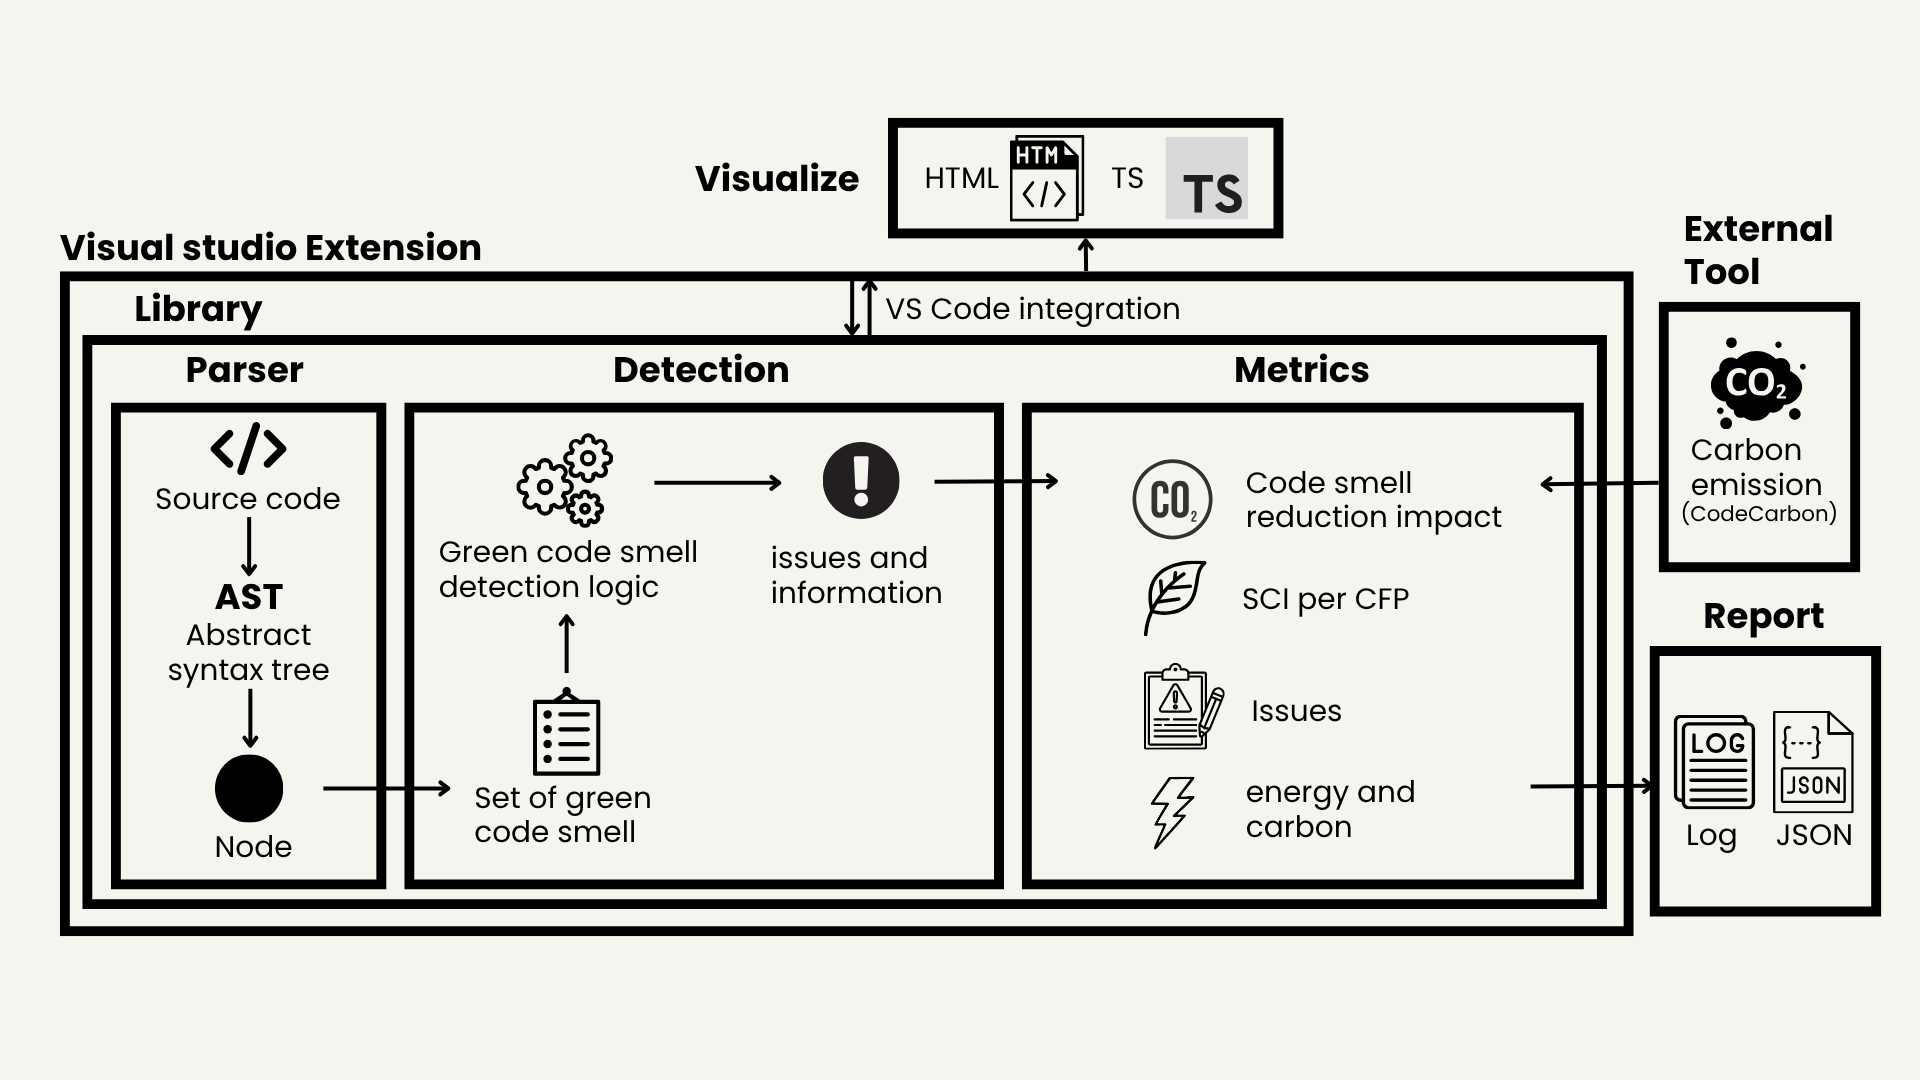
\includegraphics[width=\textwidth]{figures/chap4/Overall_SystemArchitecture.png}
\captionsetup{name=รูป}
\caption{สถาปัตยกรรมภาพรวมของระบบ PyGreenSense}
\label{fig:ch4_overall_architecture}
\end{figure}

รูป \ref{fig:ch4_overall_architecture} แสดงให้เห็นว่าตัวไลบรารีทำหน้าที่วิเคราะห์ซอร์สโค้ดและตรวจจับปัญหาเชิงโครงสร้าง ขณะที่ส่วนขยาย VS Code ทำหน้าที่เชื่อมการวิเคราะห์เข้าสู่ workflow ของผู้ใช้ และโมดูล Metrics ทำหน้าที่ประมวลผลข้อมูลด้านคาร์บอน พลังงาน CFP และผลกระทบจากการลด Code Smell เพื่อให้รายงานที่ได้มีทั้งมิติด้านคุณภาพโค้ดและความยั่งยืน

\subsection{AST Parser}
AST Parser ทำหน้าที่แปลงซอร์สโค้ดภาษา Python ให้อยู่ในรูปของโครงสร้าง {\italicfont Abstract Syntax Tree (AST)} โดยใช้โมดูล \texttt{ast} ของภาษา Python เพื่อให้สามารถวิเคราะห์องค์ประกอบของโปรแกรมในระดับโหนด เช่น ฟังก์ชัน คลาส ลูป การกำหนดค่า และการเรียกใช้ฟังก์ชันได้อย่างเป็นระบบ โครงสร้างดังกล่าวเป็นพื้นฐานสำคัญสำหรับการตรวจจับ Green Code Smell ในโครงงานนี้



\subsection{ชุดกฎ Green Code Smell}
ชุดกฎการตรวจจับถูกออกแบบขึ้นเพื่อระบุรูปแบบโค้ดที่อาจส่งผลต่อประสิทธิภาพด้านพลังงาน โดยอ้างอิงจากแนวคิดด้าน {\italicfont Green Software Engineering} งานวิจัยที่เกี่ยวข้อง และรายการ Green Code Smell ที่คัดเลือกมาใช้ในโครงงาน ได้แก่ {\italicfont Dead Code}, {\italicfont Long Method}, {\italicfont God Class}, {\italicfont Duplicated Code} และ {\italicfont Mutable Default Arguments}

\begin{table}[H]
\centering
\renewcommand{\arraystretch}{1.25}
\setlength{\tabcolsep}{6pt}
\begin{tabularx}{\textwidth}{|P{3.5cm}|X|}
\hline
{\boldfont Green Code Smell} & {\boldfont คำอธิบาย} \\
\hline
Dead Code & โค้ดที่ไม่ได้ถูกใช้งานจริง เช่น ตัวแปร ฟังก์ชัน คลาส หรือคำสั่งที่ไม่สามารถทำงานถึงได้ ({\italicfont unreachable code}) ซึ่งทำให้โค้ดมีส่วนเกินและเพิ่มภาระในการบำรุงรักษา รวมถึงอาจสะท้อนถึงการใช้ทรัพยากรที่ไม่จำเป็นในระบบ \cite{pylintUnreachable,pylintPossiblyUnusedVariable,vultureDeadCode,refactoringGuruDeadCode} \\
\hline
Long Method & ฟังก์ชันหรือเมธอดที่มีความยาวมากเกินไปและมีความซับซ้อนสูง โดยในโครงงานนี้พิจารณาจากจำนวนบรรทัดของโค้ดและค่า {\italicfont cyclomatic complexity} ซึ่งอาจทำให้โค้ดอ่านยาก ทดสอบยาก และเพิ่มภาระในการประมวลผล \cite{refactoringGuruLongMethod,guru99CyclomaticComplexity} \\
\hline
God Class & คลาสที่มีความรับผิดชอบมากเกินไป โดยในโครงงานนี้พิจารณาจากจำนวนบรรทัดของโค้ด ค่า {\italicfont cyclomatic complexity} และจำนวนเมธอดภายในคลาส ซึ่งมักสะท้อนถึงการรวมหลายหน้าที่ไว้ในคลาสเดียว \cite{refactoringGuruLargeClass,radonCyclomaticComplexity} \\
\hline
Duplicated Code & โค้ดที่มีความซ้ำคล้ายกันในหลายตำแหน่งของโปรแกรม โดยโครงงานนี้ใช้การเปรียบเทียบความคล้ายคลึงของโค้ดด้วย {\italicfont similarity threshold} เพื่อระบุกรณีที่มีการคัดลอกหรือเขียนซ้ำในลักษณะที่ใกล้เคียงกัน \cite{pythonDifflib,pylintDuplicateCode,refactoringGuruDuplicateCode} \\
\hline
Mutable Default Arguments & การกำหนดค่าเริ่มต้นของพารามิเตอร์ในฟังก์ชันเป็นชนิดข้อมูลที่เปลี่ยนแปลงได้ เช่น {\italicfont list}, {\italicfont dict} หรือ {\italicfont set} ซึ่งเป็น {\italicfont Python-specific code smell} ที่อาจทำให้เกิดพฤติกรรมไม่คาดคิดระหว่างการทำงาน \cite{pylintDangerousDefaultValue,sonarMutableDefaultArgument} \\
\hline
\end{tabularx}
\captionsetup{justification=centering, name=ตาราง}
\caption{Green Code Smell ที่สำคัญที่ใช้ในโครงการ}
\label{table:ch4_green_code_smells}
\end{table}

\subsubsection{ตรรกะการตรวจจับ Green Code Smell}
การตรวจจับ Green Code Smell ในโครงงานนี้ใช้การวิเคราะห์โครงสร้างซอร์สโค้ดภาษา Python ผ่าน Abstract Syntax Tree (AST) ร่วมกับพารามิเตอร์และเงื่อนไขที่กำหนดไว้ในแต่ละกฎ โดยแต่ละ Code Smell มีตรรกะการตรวจจับแตกต่างกันตามลักษณะของปัญหา ดังแสดงในตาราง \ref{table:ch4_detection_logic}

\begin{table}[H]
\centering
\scriptsize
\renewcommand{\arraystretch}{1.15}
\setlength{\tabcolsep}{4pt}
\begin{tabularx}{\textwidth}{|P{2.8cm}|P{3.6cm}|X|}
\hline
{\boldfont Code Smell} & {\boldfont Parameters} & {\boldfont Logic} \\
\hline

Long Method &
\texttt{max\_loc = 30}

\texttt{max\_cc = 10}
&
ตรวจสอบจำนวนบรรทัดโค้ด หรือ LOC และตรวจสอบค่าความซับซ้อนเชิงวัฏจักร หรือ Cyclomatic Complexity ของฟังก์ชัน หากจำนวนบรรทัดโค้ดหรือค่าความซับซ้อนเกินเกณฑ์ที่กำหนด ระบบจะนับเป็น Long Method \cite{refactoringGuruLongMethod,guru99CyclomaticComplexity}
\\
\hline

God Class &
\texttt{max\_cc = 35}

\texttt{max\_loc = 100}

\texttt{max\_methods = 10}
&
ตรวจสอบค่าความซับซ้อนเชิงวัฏจักร จำนวนบรรทัดโค้ด และจำนวนเมธอดภายในคลาส หากค่าใดค่าหนึ่งเกินเกณฑ์ที่กำหนด ระบบจะนับเป็น God Class \cite{refactoringGuruLargeClass,radonCyclomaticComplexity}
\\
\hline

Duplicated Code &
\texttt{similarity\_threshold = 0.85}
&
แปลงโค้ดให้อยู่ในรูปแบบมาตรฐาน เช่น แทนชื่อตัวแปรด้วย \texttt{VAR} และแทนค่าคงที่ด้วยประเภทของค่า จากนั้นเปรียบเทียบความคล้ายคลึงด้วย \texttt{difflib.SequenceMatcher} หากค่า Similarity Ratio สูงกว่า \texttt{0.85} จะนับเป็น Duplicated Code \cite{pythonDifflib,pylintDuplicateCode,refactoringGuruDuplicateCode}
\\
\hline

Dead Code &
ไม่มี parameter เฉพาะ
&
ตรวจสอบ 2 กรณีหลัก ได้แก่ Unused Variable และ Unreachable Code โดยใช้ AST เก็บข้อมูลส่วนที่ถูกประกาศและส่วนที่ถูกใช้งานจริง หากประกาศแต่ไม่ถูกใช้งานจะนับเป็น unused code และตรวจสอบคำสั่งที่ทำให้ flow สิ้นสุด เช่น \texttt{return}, \texttt{break}, \texttt{continue} และ \texttt{raise} เพื่อระบุ unreachable code \cite{pylintUnreachable,pylintPossiblyUnusedVariable,vultureDeadCode,refactoringGuruDeadCode}
\\
\hline

Mutable Default Arguments &
ไม่มี parameter เฉพาะ
&
ตรวจสอบ argument ของฟังก์ชันที่มีการกำหนดค่าเริ่มต้น และตรวจสอบว่าค่าเริ่มต้นนั้นเป็นชนิดข้อมูลที่เปลี่ยนแปลงได้หรือไม่ เช่น \texttt{list}, \texttt{dict} หรือ \texttt{set} หากพบ object ประเภทดังกล่าว ระบบจะนับเป็น Mutable Default Arguments \cite{pylintDangerousDefaultValue,sonarMutableDefaultArgument}
\\
\hline

\end{tabularx}
\captionsetup{justification=centering, name=ตาราง}
\caption{ตรรกะและพารามิเตอร์ที่ใช้ในการตรวจจับ Green Code Smell}
\label{table:ch4_detection_logic}
\end{table}

ความซับซ้อนเชิงวัฏจักร หรือ {\italicfont Cyclomatic Complexity} คือค่าที่ใช้ประเมินความซับซ้อนของเส้นทางการทำงานภายในโค้ด โดยพิจารณาจากโครงสร้างควบคุม เช่น loop, condition, \texttt{with}, list/dict/set comprehension และ operator ต่าง ๆ ยิ่งค่าดังกล่าวสูง โค้ดยิ่งมีเส้นทางการทำงานมากขึ้น และมักส่งผลให้การทดสอบ การบำรุงรักษา และการทำความเข้าใจโค้ดทำได้ยากขึ้น \cite{guru99CyclomaticComplexity,radonCyclomaticComplexity}

\subsection{VS Code Extension Module}
ส่วนขยาย VS Code ของโครงงานนี้ถูกพัฒนาขึ้นเพื่อทำหน้าที่เป็นส่วนติดต่อระหว่างผู้ใช้กับไลบรารีตรวจจับ Green Code Smell สำหรับภาษา Python โดยรองรับการเรียกใช้งานจากภายในสภาพแวดล้อมการพัฒนาโดยตรง ทำให้ผู้ใช้สามารถวิเคราะห์โค้ดและตรวจสอบผลลัพธ์ได้โดยไม่ต้องสลับไปใช้งานเครื่องมือภายนอก

ในเชิงโครงสร้าง ส่วนขยายถูกออกแบบให้มีคำสั่งหลักสำหรับการตรวจสอบสภาพแวดล้อมเสมือน การติดตั้ง dependency ที่จำเป็น การวิเคราะห์ไฟล์เดี่ยว และการวิเคราะห์ทั้งโปรเจกต์ โดยผู้ใช้สามารถเรียกใช้งานคำสั่งเหล่านี้ผ่าน Command Palette ของ VS Code ได้โดยตรง

ด้านการจัดการสภาพแวดล้อมการทำงาน ส่วนขยายใช้แนวทาง {\italicfont extension-managed virtual environment} โดยจัดเก็บ Python virtual environment ไว้ภายใต้พื้นที่จัดเก็บของส่วนขยายเอง ทำให้สามารถควบคุม dependency ที่เกี่ยวข้องกับระบบได้อย่างเป็นอิสระจากโปรเจกต์ของผู้ใช้ เมื่อระบบตรวจพบว่ายังไม่มี environment ที่พร้อมใช้งาน จะดำเนินการค้นหา system Python เพื่อใช้สร้าง virtual environment และติดตั้ง dependency ที่จำเป็นโดยอัตโนมัติ

ในการวิเคราะห์ ส่วนขยายจะตรวจสอบก่อนว่า CLI module ของ PyGreenSense สามารถเรียกใช้งานได้จริงใน environment ที่เตรียมไว้ หลังจากนั้นจึงเริ่มการวิเคราะห์ไฟล์หรือโปรเจกต์ตามขอบเขตที่ผู้ใช้เลือก โดยผลลัพธ์จากการวิเคราะห์จะถูกเก็บทั้งในรูปแบบข้อความจาก standard output และข้อมูลเชิงโครงสร้างที่บันทึกไว้ในไฟล์ \texttt{history.json} เพื่อรองรับการอ่านผลย้อนหลังและการเปรียบเทียบผลลัพธ์ระหว่างการรันแต่ละครั้ง

\subsection{Reporting Module}
โมดูลนี้ทำหน้าที่สรุปผลการตรวจสอบในรูปแบบรายงาน โดยแสดงประเภทของ Green Code Smell ตำแหน่งที่พบ ระดับความรุนแรง ค่าประมาณการใช้พลังงาน ปริมาณคาร์บอน และมาตรวัดเชิงฟังก์ชันที่เกี่ยวข้อง เช่น CFP และ SCI per CFP นอกจากนี้ยังรองรับการแสดงผลการเปรียบเทียบก่อนและหลังการปรับปรุง เพื่อช่วยให้ผู้ใช้เห็นผลของการแก้ไขโค้ดได้อย่างเป็นรูปธรรม

% -----------------------------------------------------

\section{การปฏิบัติ}

การพัฒนาโครงงานแบ่งออกเป็น 3 ระยะหลัก ได้แก่ การศึกษางานวิจัยพื้นฐาน การพัฒนาไลบรารีตรวจจับ Green Code Smell และการพัฒนาส่วนขยาย VS Code โดยมีรายละเอียดดังนี้

\subsection{ระยะการศึกษางานวิจัยและข้อมูลพื้นฐาน}
ในระยะนี้ ผู้พัฒนาได้ศึกษาทฤษฎีและงานวิจัยที่เกี่ยวข้องกับ Green Software Engineering, Code Smell, Software Carbon Intensity (SCI), CodeCarbon และ Cosmic Function Points (CFP) เพื่อใช้เป็นพื้นฐานในการออกแบบกฎตรวจจับ กลไกการวัดผล และรูปแบบการแสดงผลของระบบ

\subsection{ระยะการพัฒนาไลบรารีตรวจจับ Green Code Smell}
ในระยะนี้มีการปรับปรุงตรรกะการตรวจจับให้มีความยืดหยุ่นและแม่นยำมากขึ้น โดยประกอบด้วยการพัฒนาส่วนสำคัญดังนี้

\begin{itemize}
    \item {\boldfont Cross-file Dead Code Detection}: พัฒนาให้ระบบสามารถวิเคราะห์โหนด AST ข้ามหลายไฟล์ภายในโปรเจกต์ เพื่อประเมินสถานะการใช้งานของฟังก์ชัน ตัวแปร หรือองค์ประกอบอื่น ๆ ในระดับโปรเจกต์

    \item {\boldfont Enhanced Duplicated Code Logic}: ปรับปรุงอัลกอริทึมการเปรียบเทียบโครงสร้าง AST เพื่อให้สามารถตรวจจับโค้ดซ้ำได้แม่นยำขึ้น แม้จะมีการเปลี่ยนชื่อของตัวแปรหรือพารามิเตอร์

    \item {\boldfont Carbon-Smell Breakdown Engine}: พัฒนาระบบประมวลผลข้อมูลเพื่อคำนวณและเปรียบเทียบสัดส่วนผลกระทบของ Green Code Smell แต่ละประเภทตามสูตร Estimated Saving
\end{itemize}

ภาพรวมของ workflow ภายในไลบรารีแสดงในรูป \ref{fig:ch4_library_workflow} ซึ่งชี้ให้เห็นว่าขั้นตอนการทำงานเริ่มจากการรับซอร์สโค้ด การ parse และวิเคราะห์โครงสร้าง ก่อนวิ่งผ่านชุดกฎตรวจจับทีละประเภทและสรุปผลร่วมกับ metric ที่เกี่ยวข้อง

\begin{figure}[H]
\centering
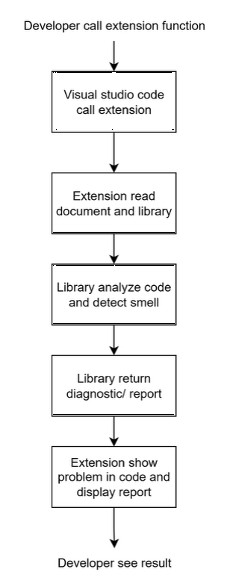
\includegraphics[width=0.45\textwidth]{figures/chap4/Process_Library.jpg}
\captionsetup{name=รูป}
\caption{Workflow การทำงานของไลบรารี PyGreenSense}
\label{fig:ch4_library_workflow}
\end{figure}

\subsection{ระยะการพัฒนาส่วนขยาย VS Code}
เมื่อไลบรารีตรวจจับพร้อมใช้งานแล้ว จึงพัฒนาส่วนขยาย VS Code เพื่อให้ผู้ใช้สามารถเข้าถึงผลการวิเคราะห์ได้สะดวกและตีความผลลัพธ์ได้ง่ายขึ้น โดยมีการพัฒนาสำคัญดังนี้

\begin{itemize}
    \item {\boldfont Library Deployment}
    
    เชื่อมต่อส่วนขยายกับไลบรารีที่ใช้งานจริงผ่านกลไก command bridge เพื่อให้ Extension สามารถสั่งรันโมดูลวิเคราะห์ รับค่าผลลัพธ์จากระบบตรวจจับ และดึงข้อมูลจากโมดูล Metric and Analysis ได้โดยตรง

    \item {\boldfont Advanced Visualization Dashboard}
    
    ออกแบบการแสดงผลข้อมูลจากไฟล์ JSON ให้อยู่ในรูปแบบ dashboard ที่เข้าใจง่าย เช่น กราฟเปรียบเทียบผลก่อนและหลังการปรับปรุง ({\italicfont Before vs After}) และแผนภูมิสัดส่วนผลกระทบรายประเภทของ Code Smell
\end{itemize}

ลำดับการทำงานของส่วนขยาย VS Code แสดงในรูป \ref{fig:ch4_extension_workflow} โดยผู้ใช้เริ่มต้นจากการเรียกคำสั่งของ Extension จากนั้นส่วนขยายจะอ่านเอกสารและเรียกใช้ไลบรารีเพื่อวิเคราะห์โค้ด ก่อนนำผลลัพธ์กลับมาแสดงทั้งในรูปแบบปัญหาบนโค้ดและรายงานสรุปภายใน VS Code

\begin{figure}[H]
\centering
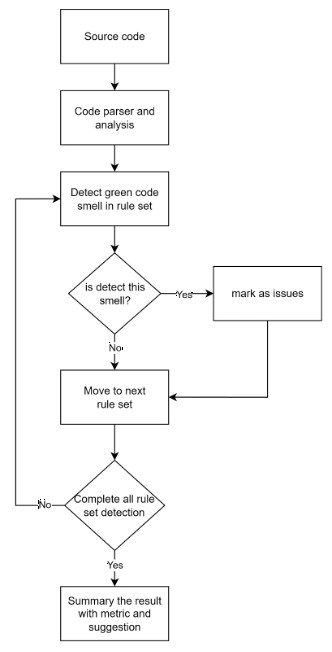
\includegraphics[width=0.32\textwidth]{figures/chap4/Process_VisualCodeExtension.jpg}
\captionsetup{name=รูป}
\caption{Workflow การทำงานของส่วนขยาย VS Code}
\label{fig:ch4_extension_workflow}
\end{figure}

% -----------------------------------------------------

\section{การทดสอบระบบ}

การทดสอบระบบมีวัตถุประสงค์เพื่อประเมินความถูกต้อง ความเสถียร และความเหมาะสมในการใช้งานจริงของทั้งไลบรารีและส่วนขยาย VS Code โดยแบ่งการทดสอบออกเป็นหลายด้านดังนี้

\subsection{การทดสอบไลบรารี}
มุ่งเน้นการทดสอบความถูกต้องของกฎตรวจจับ Green Code Smell แต่ละประเภท รวมถึงการทำงานร่วมกันของโมดูล AST Parser, Detection Rules และโมดูลคำนวณผลลัพธ์

\subsection{การทดสอบส่วนขยาย VS Code}
มุ่งเน้นการประเมินประสบการณ์ผู้ใช้ ความถูกต้องของข้อมูลที่แสดงผล และความสามารถในการเชื่อมต่อกับไลบรารีและระบบบันทึกผล

\subsection{การทดสอบด้านมาตรวัด}
ในส่วนนี้เน้นการตรวจสอบความถูกต้องของตรรกะการคำนวณมาตรวัดเชิงฟังก์ชัน มาตรวัดความเข้มข้นคาร์บอน และผลกระทบด้านการลดคาร์บอน โดยแยกการทดสอบออกเป็น 4 ส่วนสำคัญ เพื่อไม่ให้ตรรกะ CFP และ SCI ปะปนกับตรรกะการคำนวณสัดส่วน Carbon Saving ดังนี้

\begin{itemize}
    \item {\boldfont CFP Measurement Test}
    
    ทดสอบความถูกต้องของตรรกะการนับหน่วยฟังก์ชันของซอฟต์แวร์ หรือ Cosmic Function Points (CFP) โดยพิจารณาจากการระบุและนับจำนวนการเคลื่อนย้ายข้อมูล ({\italicfont Data Movements}) ได้แก่ Entry, Exit, Read และ Write เพื่อประเมินว่าระบบสามารถประมาณค่าขนาดเชิงฟังก์ชันของซอฟต์แวร์จากซอร์สโค้ดได้อย่างเหมาะสม

    \item {\boldfont SCI per CFP Measurement Test}
    
    ทดสอบตรรกะการคำนวณค่า Software Carbon Intensity ต่อหน่วย CFP หรือ {\italicfont SCI per CFP} โดยพิจารณาความสัมพันธ์ระหว่างปริมาณคาร์บอนที่ปล่อยออกมาและจำนวนหน่วยฟังก์ชันที่ระบบประมาณได้ เพื่อประเมินความเข้มข้นของคาร์บอนต่อหน่วยงานที่ซอฟต์แวร์ทำจริง

    \item {\boldfont Carbon Saving Impact Analysis Test}
    
    ทดสอบตรรกะการคำนวณสัดส่วนการประหยัดคาร์บอนจากข้อมูลที่จัดเก็บใน History Log โดยเปรียบเทียบข้อมูลก่อนและหลังการปรับปรุงโค้ด เช่น ปริมาณคาร์บอนรวม จำนวน Code Smell ที่ลดลง และจำนวนบรรทัดของโค้ดที่ถูกลบหรือปรับปรุงออกจากแต่ละกฎ เพื่อนำไปใช้ประเมินผลกระทบของการกำจัด Green Code Smell ต่อการลดปริมาณคาร์บอนในภาพรวม

    \item {\boldfont Inversion Case Handling}
    
    วิเคราะห์กรณีที่จำนวน CFP ลดลงในสัดส่วนที่มากกว่าปริมาณคาร์บอนที่ลดลง ซึ่งอาจทำให้ค่า SCI ต่อหน่วยสูงขึ้น แม้ว่าปริมาณคาร์บอนรวมจะลดลงก็ตาม กรณีนี้ใช้เพื่อตรวจสอบว่าระบบสามารถอธิบายผลลัพธ์ที่ดูขัดแย้งกันระหว่างคาร์บอนรวมและคาร์บอนต่อหน่วยฟังก์ชันได้อย่างถูกต้อง
\end{itemize}

ผลลัพธ์จากการทดสอบทั้ง 4 ส่วนถูกนำไปใช้กำหนดตรรกะการแสดงผลของระบบในบทประเมินผล โดยเฉพาะกรณี {\italicfont Inversion Case} ซึ่งช่วยให้ระบบอธิบายสถานการณ์ที่จำนวน Code Smell และ CFP ลดลง แต่ค่า SCI ต่อหน่วยกลับเพิ่มขึ้นได้อย่างเป็นระบบมากขึ้น ทั้งนี้ตัวอย่างผลการเปรียบเทียบจากการทดสอบจริงของไลบรารี ส่วนขยาย และข้อมูลจาก history log จะนำเสนอเพิ่มเติมในบทที่ \ref{Ch:Evaluation}

    \clearpage

    \chapter{การประเมินผล}
\label{Ch:Evaluation}

การประเมินผลของระบบ {\italicfont PyGreenSense} มุ่งเน้นการตรวจสอบทั้งในระดับไลบรารีสำหรับตรวจจับ {\italicfont Green Code Smell} และในระดับส่วนขยาย {\italicfont Visual Studio Code (VS Code Extension)} เพื่อประเมินความถูกต้อง ความน่าเชื่อถือ และความเหมาะสมในการใช้งานจริงของระบบ โดยแนวทางการประเมินแบ่งออกเป็น 2 ส่วนหลัก ได้แก่ (1) การประเมินผลไลบรารี และ (2) การประเมินผลส่วนขยาย VS Code

นอกจากนี้ แนวทางการประเมินยังพิจารณาใน 3 มิติสำคัญ ได้แก่ การเปรียบเทียบผลก่อนและหลังใช้งานในด้านพลังงาน การเปรียบเทียบผลกับเครื่องมือที่ใกล้เคียง และการวัดผลจากการใช้งานจริงของผู้ใช้

% -----------------------------------------------------

\section{การประเมินผลไลบรารี}

การประเมินผลในระดับไลบรารีมีวัตถุประสงค์เพื่อพิสูจน์ว่าระบบตรวจจับ {\italicfont Green Code Smell} ที่พัฒนาขึ้นสามารถทำงานได้อย่างมีประสิทธิภาพในสถานการณ์ที่ใกล้เคียงกับการใช้งานจริง โดยเน้นการเปรียบเทียบความสามารถในการตรวจจับกับเครื่องมือที่เป็นที่รู้จักในอุตสาหกรรม เพื่อสร้างความเชื่อมั่นต่อผลการวิเคราะห์ของระบบ

\subsection{ชุดข้อมูลและเครื่องมือที่ใช้ในการทดสอบ}

ในการประเมินผลครั้งนี้ ใช้ซอร์สโค้ดภาษา Python ขนาดประมาณ 5{,}000 บรรทัด (LOC) เพื่อจำลองลักษณะของโปรเจกต์ที่มีความซับซ้อนในระดับการใช้งานจริง โดยเลือกเครื่องมืออ้างอิงสำหรับการเปรียบเทียบดังนี้

\begin{itemize}
    \item {\boldfont Vulture} สำหรับการตรวจจับ {\italicfont Dead Code}
    \item {\boldfont PyExamine} สำหรับการตรวจจับ {\italicfont Long Method} และ {\italicfont Large Class (God Class)}
    \item {\boldfont Smell-detector-python} สำหรับการตรวจจับ {\italicfont Long Method}
\end{itemize}

แนวทางดังกล่าวช่วยให้สามารถเปรียบเทียบความสามารถของ {\boldfont PyGreenSense} กับเครื่องมือเฉพาะทางที่มีการใช้งานอยู่แล้ว และช่วยยืนยันว่า {\italicfont logic} การตรวจจับของระบบมีความสอดคล้องกับแนวทางมาตรฐานในงานวิเคราะห์โค้ด

\subsection{ผลการเปรียบเทียบการตรวจจับ Code Smell}

การทดสอบเชิงเปรียบเทียบ ({\boldfont Benchmarking}) ถูกใช้เพื่อประเมินว่า {\boldfont PyGreenSense} สามารถตรวจจับ {\italicfont Green Code Smell} แต่ละประเภทได้ครอบคลุมและมีความสอดคล้องกับเครื่องมืออ้างอิงเพียงใด โดยการประเมินในส่วนนี้ครอบคลุมอย่างน้อยปัญหาสำคัญ เช่น {\boldfont Dead Code}, {\boldfont Long Method} และ {\boldfont God Class} ซึ่งเป็น {\italicfont code smell} ที่มีความสัมพันธ์กับคุณภาพของโค้ดและอาจส่งผลต่อพลังงานของซอฟต์แวร์ได้ \cite{verdecchia2018energy}

ผลการประเมินในมิตินี้พิจารณาจากประเด็นสำคัญดังต่อไปนี้

\begin{itemize}
    \item จำนวนปัญหาที่ระบบตรวจพบในแต่ละประเภท
    \item ความสอดคล้องของผลลัพธ์กับเครื่องมืออ้างอิง
    \item กรณีที่ระบบตรวจพบเพิ่มเติมจากเครื่องมืออ้างอิง หรือกรณีที่มีความแตกต่างในการตีความ
    \item ความสามารถในการตรวจจับ {\italicfont smell} ที่สัมพันธ์กับบริบทด้าน {\italicfont Green Software Engineering}
\end{itemize}

\begin{table}[H]
    \centering
    \begin{tabularx}{\textwidth}{>{\raggedright\arraybackslash}p{3cm} >{\raggedright\arraybackslash}p{4cm} X}
        \toprule
        {\boldfont ประเภท Code Smell} & {\boldfont ผลการเปรียบเทียบ (Benchmarking)} & {\boldfont หมายเหตุ} \\
        \midrule
        Dead Code
        & ตรงกันกับเครื่องมือ Vulture
        & ตรวจพบฟังก์ชันและตัวแปรที่ไม่ได้ใช้งานได้อย่างแม่นยำ \\
        Long Method
        & ตรงกันกับ PyExamine และ smell-detector-python
        & มีการคำนวณจำนวนบรรทัดในฟังก์ชันที่สอดคล้องกัน \\
        God Class
        & ตรงกันกับ PyExamine
        & ตรวจจับคลาสที่มีขนาดใหญ่เกินไป ({\italicfont Large Class}) ได้อย่างถูกต้อง \\
        Duplicated Code
        & มีความแตกต่างในด้านขอบเขตการตรวจจับ
        & เครื่องมืออื่นมักตรวจแบบข้ามไฟล์ ({\italicfont Cross-file}) แต่ในเวอร์ชันปัจจุบันของ {\italicfont PyGreenSense} เน้นการตรวจภายในไฟล์เดียวกัน ({\italicfont Single-file}) \\
        Mutable Default Argument
        & ตรวจสอบด้วยตนเอง ({\italicfont Manual})
        & เนื่องจากไม่พบเครื่องมืออัตโนมัติที่รองรับกฎนี้ จึงใช้วิธีนับบรรทัดที่มีการประกาศ \texttt{list}/\texttt{dict} ในพารามิเตอร์ฟังก์ชัน \\
        \bottomrule
    \end{tabularx}
\captionsetup{justification=centering, name=ตาราง}
\caption{ผลการเปรียบเทียบการตรวจจับ Code Smell}
\label{tab:benchmark-smells}
\end{table}

\subsection{ตัวอย่างผลการเปรียบเทียบกับเครื่องมืออ้างอิง}

นอกจากผลในตาราง \ref{tab:benchmark-smells} แล้ว ผู้จัดทำยังรวบรวมตัวอย่างผลลัพธ์จากการรันจริงเพื่อเปรียบเทียบรูปแบบการรายงานของ {\italicfont PyGreenSense} กับเครื่องมืออ้างอิงในแต่ละกรณีศึกษา ดังรูป \ref{fig:ch5_deadcode_benchmark} ถึงรูป \ref{fig:ch5_godclass_benchmark}

\begin{figure}[H]
    \centering
    \begin{subfigure}[t]{0.48\textwidth}
        \centering
        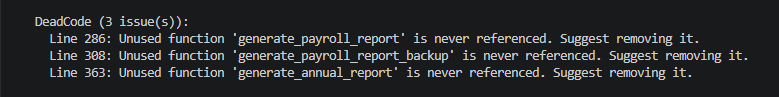
\includegraphics[width=\textwidth]{figures/chap5/benchmark_deadcode_pygreensense.png}
        \captionsetup{name=รูป}
        \caption{ผลจาก PyGreenSense}
    \end{subfigure}
\hfill
\begin{subfigure}[t]{0.48\textwidth}
    \centering
    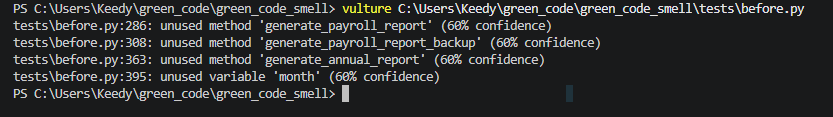
\includegraphics[width=\textwidth]{figures/chap5/benchmark_deadcode_vulture.png}
    \captionsetup{name=รูป}
    \caption{ผลจาก Vulture}
\end{subfigure}
\captionsetup{name=รูป}
\caption{ตัวอย่างการเปรียบเทียบการตรวจจับ Dead Code ระหว่าง PyGreenSense และ Vulture}
\label{fig:ch5_deadcode_benchmark}
\end{figure}

\begin{figure}[H]
    \centering
    \begin{subfigure}[t]{0.48\textwidth}
        \centering
        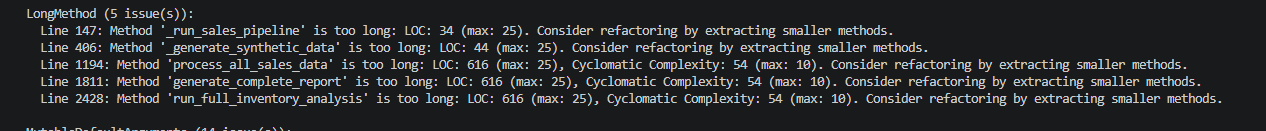
\includegraphics[width=\textwidth]{figures/chap5/benchmark_longmethod_pygreensense.png}
        \captionsetup{name=รูป}
        \caption{ผลจาก PyGreenSense}
    \end{subfigure}
\hfill
\begin{subfigure}[t]{0.48\textwidth}
    \centering
    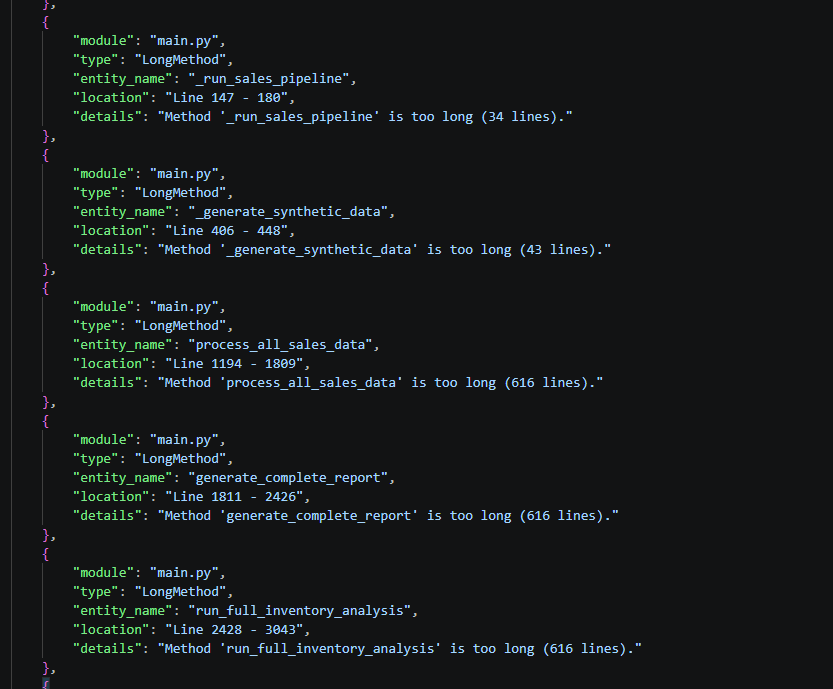
\includegraphics[width=\textwidth]{figures/chap5/benchmark_longmethod_smell_detector.png}
    \captionsetup{name=รูป}
    \caption{ผลจาก Smell-detector-python}
\end{subfigure}
\captionsetup{name=รูป}
\caption{ตัวอย่างการเปรียบเทียบการตรวจจับ Long Method ระหว่าง PyGreenSense และ Smell-detector-python}
\label{fig:ch5_longmethod_benchmark}
\end{figure}

\begin{figure}[H]
    \centering
    \begin{subfigure}[t]{0.76\textwidth}
        \centering
        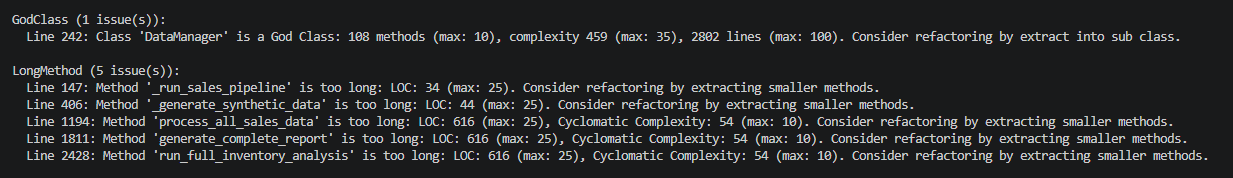
\includegraphics[width=\textwidth]{figures/chap5/benchmark_godclass_pygreensense.png}
        \captionsetup{name=รูป}
        \caption{ผลจาก PyGreenSense}
    \end{subfigure}
\hfill
\begin{subfigure}[t]{0.18\textwidth}
    \centering
    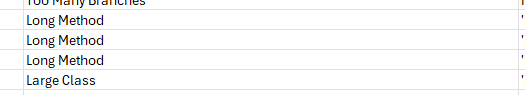
\includegraphics[width=\textwidth]{figures/chap5/benchmark_godclass_pyexamine.png}
    \captionsetup{name=รูป}
    \caption{ผลจาก PyExamine}
\end{subfigure}
\captionsetup{name=รูป}
\caption{ตัวอย่างการเปรียบเทียบการตรวจจับ God Class ระหว่าง PyGreenSense และ PyExamine}
\label{fig:ch5_godclass_benchmark}
\end{figure}

จากรูปข้างต้นจะเห็นว่า {\italicfont PyGreenSense} สามารถรายงานปัญหาในรูปแบบที่อ่านง่ายและเชื่อมโยงกับรายละเอียดเชิงโครงสร้างของโค้ดได้ชัดเจน ขณะที่เครื่องมืออ้างอิงบางตัวอาจรายงานผลในรูปแบบข้อความหรือไฟล์ข้อมูลที่ต่างกัน เช่น {\italicfont PyExamine} ที่แสดงผลเชิงตาราง/CSV และ {\italicfont Smell-detector-python} ที่แสดงผลเชิง JSON หรือ log ทั้งนี้จำนวน smell ที่ตรวจพบอาจไม่เท่ากันทุกเครื่องมือเนื่องจากแต่ละระบบใช้ threshold และตรรกะการตีความปัญหาที่ต่างกัน

\subsection{การวิเคราะห์ผลในระดับไลบรารี}

ในมิติของไลบรารี จุดเด่นของ {\italicfont PyGreenSense} ไม่ได้จำกัดอยู่เพียงการตรวจจับ {\italicfont code smell} แบบทั่วไปเท่านั้น แต่ยังมุ่งเชื่อมโยงผลการตรวจจับเข้ากับแนวคิดด้านพลังงานและความยั่งยืนของซอฟต์แวร์ ซึ่งสอดคล้องกับกรอบแนวคิดของ {\italicfont Green Software Engineering} และ {\italicfont Green Code Smells} \cite{leGoaer2024tactics,legoaer2023ecocode} ผลลัพธ์ที่ได้จากไลบรารีจึงมีความเหมาะสมสำหรับใช้เป็นฐานข้อมูลในการวิเคราะห์ต่อยอดด้านคาร์บอน พลังงาน และตัวชี้วัดเชิงฟังก์ชันในขั้นถัดไป

% -----------------------------------------------------

\section{การประเมินผลจากชุดโค้ดทดสอบ}

การประเมินผลจากชุดโค้ดทดสอบมีวัตถุประสงค์เพื่อพิจารณาว่า การตรวจจับและการปรับปรุงโค้ดตามแนวทางของ {\italicfont PyGreenSense} สามารถสะท้อนผลลัพธ์ในเชิงโครงสร้างของโค้ด มาตรวัดเชิงฟังก์ชัน และค่าพลังงานหรือคาร์บอนได้อย่างไร โดยอ้างอิงจากข้อมูลการทดลองในเอกสารประกอบส่วน {\italicfont Evaluation}

\subsection{Source Code สำหรับการประเมิน}

ในการศึกษานี้ ชุด {\italicfont source code} ที่ใช้ในการทดลองเป็นโปรแกรมภาษา Python ที่สร้างขึ้นด้วย {\italicfont generative AI} เนื่องจากไม่สามารถหาโปรเจกต์ที่มี {\italicfont code smell} ครบทั้ง 5 ประเภทตามกฎที่กำหนดได้ ชุดข้อมูลจึงถูกแบ่งออกเป็น 4 ระดับขนาดเพื่อสะท้อนความซับซ้อนของโค้ดที่แตกต่างกัน ได้แก่

\begin{itemize}
    \item {\boldfont Micro scale}: ประมาณ 500 บรรทัด (LOC)
    \item {\boldfont Small scale}: ประมาณ 3{,}000 บรรทัด
    \item {\boldfont Medium scale}: ประมาณ 5{,}000 บรรทัด
    \item {\boldfont Large scale}: ประมาณ 10{,}000 บรรทัด
\end{itemize}

โดยในแต่ละชุดข้อมูลถูกออกแบบให้มี {\italicfont code smell} ครบทั้ง 5 ประเภท ได้แก่ {\italicfont God Class}, {\italicfont Long Method}, {\italicfont Duplicated Code}, {\italicfont Dead Code} และ {\italicfont Mutable Default Arguments} การตั้งค่าเช่นนี้ช่วยให้สามารถประเมินประสิทธิภาพของการตรวจจับ {\italicfont code smell} ได้อย่างเป็นระบบในสภาวะที่ควบคุมได้ และสามารถเปรียบเทียบผลลัพธ์ระหว่างโค้ดที่มีขนาดแตกต่างกันได้อย่างชัดเจน

\subsection{สรุปผลจากการ Refactor}

จากการทดลองกับชุดโค้ดที่มีขนาดแตกต่างกัน ได้แก่ Micro, Small, Medium และ Large พบประเด็นสำคัญดังนี้

\begin{itemize}
    \item การ refactor ช่วยลดจำนวน Code Smell หรือปัญหาเชิงโครงสร้างของโค้ดได้ในทุกขนาดของโปรเจกต์
    \item ผลลัพธ์ด้านคาร์บอนมีความหลากหลายตามขนาดโปรเจกต์ โดยในชุด Micro และ Small มีแนวโน้มดีขึ้น แต่ใน Medium และ Large ค่าคาร์บอนกลับแย่ลงเล็กน้อย ทั้งนี้อาจเป็นเพราะการ refactor ในโปรเจกต์ขนาดใหญ่มักเพิ่ม {\italicfont abstraction layer} มากขึ้น ทำให้เกิด {\italicfont runtime overhead} สะสมจนมีนัยสำคัญ ขณะที่โปรเจกต์ขนาดเล็กยังได้รับประโยชน์จากการ refactor มากกว่าเพราะ {\italicfont overhead} ที่เพิ่มขึ้นยังน้อยกว่าผลดีที่ได้รับ
    \item ค่า CFP ลดลงในทุกกรณี แสดงให้เห็นว่าโค้ดหลังการ refactor มีขนาดเชิงฟังก์ชันที่เล็กลง อย่างไรก็ตาม ค่า SCI/CFP กลับเพิ่มสูงขึ้น อาจเกิดจากข้อจำกัดของการคำนวณ SCI กล่าวคือเมื่อ refactor แล้วค่าคาร์บอนจริงลดลงเพียงเล็กน้อย แต่ CFP ลดลงมาก เมื่อนำมาหารกันจึงทำให้ค่า SCI/CFP เพิ่มขึ้น แม้ว่าจำนวน Code Smell และ CFP โดยรวมจะลดลงก็ตาม
    \item ผลลัพธ์ของชุดข้อมูลขนาด Large มีความน่าเชื่อถือน้อยกว่าขนาดอื่น เนื่องจากใช้จำนวนการทดสอบน้อยกว่า และมีภาระงานระหว่างการรันหรือ runtime overhead สูงกว่า
    \item โดยสรุป การ refactor ช่วยให้โค้ดดูแลรักษาง่ายขึ้นอย่างชัดเจน แต่ผลกระทบด้านคาร์บอนขึ้นอยู่กับขนาดของโปรเจกต์ สภาพแวดล้อมการทดสอบ และลักษณะงานที่เกิดขึ้นระหว่างการรัน จึงไม่สามารถสรุปได้ว่าการ refactor จะทำให้ค่าคาร์บอนดีขึ้นเสมอไป
\end{itemize}

\subsection{ผลลัพธ์เชิงปริมาณจากชุดโค้ดทดสอบ}

ตาราง \ref{tab:evaluation-result-metrics} แสดงผลลัพธ์เชิงปริมาณจากชุดโค้ดทดสอบ โดยค่าที่แสดงในรูปแบบ ``ก่อน/หลัง'' หมายถึงค่าก่อนการ refactor และหลังการ refactor ตามลำดับ

\begin{table}[H]
    \centering
    \scriptsize
    \renewcommand{\arraystretch}{1.15}
    \setlength{\tabcolsep}{3pt}
    \begin{tabularx}{\textwidth}{|P{2.1cm}|P{2.2cm}|P{2.5cm}|P{2.5cm}|P{2.5cm}|X|}
        \hline
        {\boldfont ขนาดชุดทดสอบ} & {\boldfont CFP ก่อน/หลัง} & {\boldfont Emissions ก่อน/หลัง (kg CO$_2$)} & {\boldfont Energy ก่อน/หลัง (kWh)} & {\boldfont LOC ก่อน/หลัง} & {\boldfont การตีความผลลัพธ์} \\
        \hline
        Micro (ประมาณ 500 LOC) & 167 / 55 & 2.52e-07 / 2.21e-07 & 4.59e-07 / 4.02e-07 & 722 / 346 & Code Smell, CFP, emissions และ energy ลดลงหลังการ refactor \\
        \hline
        Small (ประมาณ 2{,}500 LOC) & 548 / 30 & 9.60e-06 / 7.18e-07 & 1.75e-05 / 1.31e-06 & 6{,}260 / 548 & ผลลัพธ์หลัง refactor ดีขึ้นชัดเจนทั้งด้านโครงสร้างและค่าคาร์บอน \\
        \hline
        Medium (ประมาณ 5{,}000 LOC) & 1010.5 / 134.5 & 1.18e-06 / 1.25e-06 & 2.24e-06 / 2.28e-06 & 8{,}640.4 / 1{,}011.6 & Code Smell และ CFP ลดลง แต่ emissions และ energy เพิ่มขึ้นเล็กน้อย \\
        \hline
        Large (ประมาณ 10K LOC) & 1489 / 1000.7 & 4.42e-06 / 4.50e-06 & 4.33e-06 / 4.43e-06 & 21{,}258 / 14{,}174.0 & โค้ดหลัง refactor มีขนาดลดลง แต่ค่าคาร์บอนและพลังงานสูงขึ้นเล็กน้อย และมีข้อจำกัดด้านจำนวนรอบการทดสอบ \\
        \hline
    \end{tabularx}
\captionsetup{justification=centering, name=ตาราง}
\caption{ผลลัพธ์เชิงปริมาณก่อนและหลังการ refactor จากชุดโค้ดทดสอบ}
\label{tab:evaluation-result-metrics}
\end{table}

\subsection{ผลลัพธ์การตรวจจับ Code Smell ในแต่ละขนาดของโปรเจกต์}

ตาราง \ref{tab:evaluation-smell-counts} แสดงจำนวน Code Smell ที่ตรวจพบในแต่ละขนาดของโปรเจกต์ โดยตัวเลขในแต่ละช่องแสดงผลในรูปแบบ ``ก่อน/หลัง'' เช่นเดียวกับตารางก่อนหน้า

\begin{table}[H]
    \centering
    \scriptsize
    \renewcommand{\arraystretch}{1.15}
    \setlength{\tabcolsep}{3pt}
    \begin{tabularx}{\textwidth}{|P{2.0cm}|P{2.0cm}|P{2.4cm}|P{2.2cm}|P{2.0cm}|X|}
        \hline
        {\boldfont ขนาดชุดทดสอบ} & {\boldfont God Class} & {\boldfont Duplicated Code} & {\boldfont Long Method} & {\boldfont Dead Code} & {\boldfont Mutable Default Arguments} \\
        \hline
        Micro & 1 / 1 & 5 / 1 & 2 / 2 & 9 / 0 & 6 / 0 \\
        \hline
        Small & 1 / 0 & 7 / 1 & 5 / 1 & 109 / 0 & 14 / 0 \\
        \hline
        Medium & 0.9 / 0.1 & 7.2 / 0.8 & 3.7 / 1.3 & 88.2 / 9.8 & 97.2 / 10.8 \\
        \hline
        Large & 1 / 0.67 & 14 / 10 & 7 / 4.67 & 118 / 78.67 & 142 / 94.67 \\
        \hline
    \end{tabularx}
\captionsetup{justification=centering, name=ตาราง}
\caption{จำนวน Code Smell ที่ตรวจพบก่อนและหลังการ refactor ในแต่ละขนาดของโปรเจกต์}
\label{tab:evaluation-smell-counts}
\end{table}

ผลลัพธ์จากตาราง \ref{tab:evaluation-result-metrics} และตาราง \ref{tab:evaluation-smell-counts} แสดงให้เห็นว่า การ refactor มีผลโดยตรงต่อการลดจำนวน Code Smell และจำนวนบรรทัดของโค้ดในทุกขนาดของชุดทดสอบ โดยเฉพาะในชุด Micro และ Small ที่ค่าพลังงานและคาร์บอนลดลงหลังการ refactor อย่างไรก็ตาม ในชุด Medium และ Large แม้จำนวน Code Smell และ CFP จะลดลง แต่ค่าคาร์บอนและพลังงานกลับเพิ่มขึ้นเล็กน้อย ซึ่งอาจเกิดจากปัจจัยภายนอก เช่น overhead ระหว่างการรัน สภาพแวดล้อมของเครื่องทดสอบ หรือความผันผวนของการวัดในระดับพลังงานต่ำมาก ดังนั้น ผลลัพธ์ด้านคาร์บอนจึงควรตีความร่วมกับจำนวนรอบการทดสอบ ขนาดของโปรเจกต์ และบริบทการทำงานของโค้ด

\subsection{ตัวอย่างผลก่อนและหลังการ refactor}

เพื่อให้เห็นผลของการปรับปรุงโค้ดในระดับกรณีศึกษา รูป \ref{fig:ch5_godclass_refactor} และรูป \ref{fig:ch5_duplicate_refactor} แสดงตัวอย่างผลก่อนและหลังการ refactor ของปัญหา {\italicfont God Class} และ {\italicfont Duplicated Code} ตามลำดับ ซึ่งช่วยยืนยันว่าระบบสามารถใช้ติดตามผลการลด Code Smell ได้จริงในระดับไฟล์ทดสอบ

\begin{figure}[H]
    \centering
    \begin{subfigure}[t]{0.48\textwidth}
        \centering
        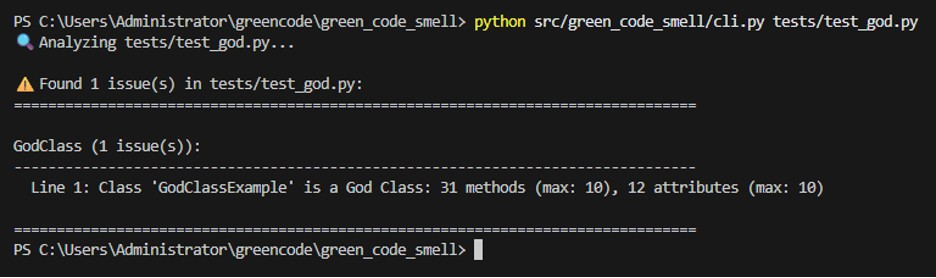
\includegraphics[width=\textwidth]{figures/chap5/godclass_before_refactor.jpg}
        \captionsetup{name=รูป}
        \caption{ก่อนการ refactor}
    \end{subfigure}
\hfill
\begin{subfigure}[t]{0.48\textwidth}
    \centering
    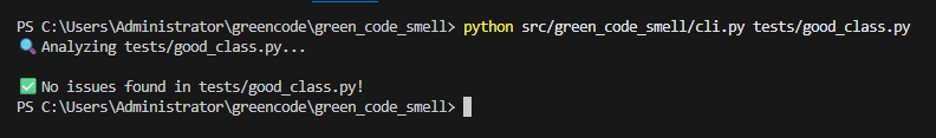
\includegraphics[width=\textwidth]{figures/chap5/godclass_after_refactor.jpg}
    \captionsetup{name=รูป}
    \caption{หลังการ refactor}
\end{subfigure}
\captionsetup{name=รูป}
\caption{ตัวอย่างผลการตรวจจับ God Class ก่อนและหลังการ refactor}
\label{fig:ch5_godclass_refactor}
\end{figure}

\begin{figure}[H]
    \centering
    \begin{subfigure}[t]{0.48\textwidth}
        \centering
        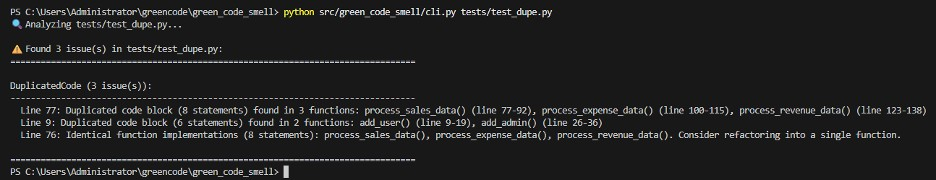
\includegraphics[width=\textwidth]{figures/chap5/duplicated_before_refactor.jpg}
        \captionsetup{name=รูป}
        \caption{ก่อนการ refactor}
    \end{subfigure}
\hfill
\begin{subfigure}[t]{0.48\textwidth}
    \centering
    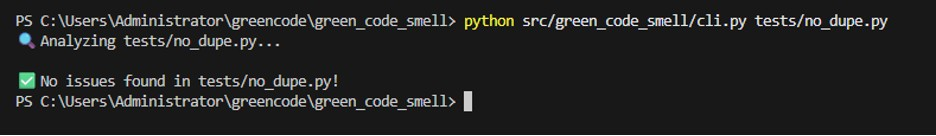
\includegraphics[width=\textwidth]{figures/chap5/duplicated_after_refactor.jpg}
    \captionsetup{name=รูป}
    \caption{หลังการ refactor}
\end{subfigure}
\captionsetup{name=รูป}
\caption{ตัวอย่างผลการตรวจจับ Duplicated Code ก่อนและหลังการ refactor}
\label{fig:ch5_duplicate_refactor}
\end{figure}

จากตัวอย่างดังกล่าวจะเห็นว่าหลังการ refactor จำนวนปัญหาที่ระบบตรวจพบลดลงอย่างชัดเจน และข้อความแสดงผลมีความตรงไปตรงมามากขึ้นต่อผู้ใช้ ช่วยให้การติดตามผลก่อนและหลังการแก้ไขสามารถทำได้ทั้งในเชิงคุณภาพและเชิงปริมาณ

% -----------------------------------------------------

\section{การประเมินผลส่วนขยาย VS Code}

การประเมินผลในระดับส่วนขยาย VS Code มีวัตถุประสงค์เพื่อทดสอบว่าระบบสามารถนำผลการวิเคราะห์จากไลบรารีมาใช้งานภายใน {\italicfont workflow} ของนักพัฒนาได้จริงหรือไม่ โดยพิจารณาทั้งด้านความถูกต้องของข้อมูลที่แสดงผล ความสะดวกในการใช้งาน และความสามารถในการนำเสนอผลวิเคราะห์ในรูปแบบที่เข้าใจง่ายสำหรับผู้ใช้ปลายทาง

\subsection{ขอบเขตการประเมินผลของ Extension}

จากโค้ดของส่วนขยาย ระบบรองรับคำสั่งหลักสำหรับการตรวจสอบ {\italicfont virtual environment} การติดตั้ง {\italicfont dependency} การวิเคราะห์ไฟล์เดี่ยว และการวิเคราะห์ทั้งโปรเจกต์ นอกจากนี้ยังสามารถเปิดผลการวิเคราะห์ผ่าน {\italicfont Webview Panel} ภายใน VS Code ได้โดยตรง

การประเมินผลของส่วนขยายจึงครอบคลุมประเด็นสำคัญดังต่อไปนี้

\begin{itemize}
    \item ความถูกต้องของการเชื่อมต่อระหว่าง Extension กับไลบรารี Python
    \item ความสามารถในการจัดการ {\italicfont environment} และ {\italicfont dependency}
    \item ความสมบูรณ์ของข้อมูลที่อ่านจาก \texttt{history.json} และผลลัพธ์จากการรันจริง
    \item ความเหมาะสมของการแสดงผลผ่าน {\italicfont Webview Dashboard}
\end{itemize}

\subsection{ผลการแสดงผลและการรายงานผลผ่าน Webview}

จาก {\italicfont implementation} ของส่วนขยาย ระบบมีการเตรียมสภาพแวดล้อม Python ผ่าน extension venv ตรวจสอบว่า CLI ของ PyGreenSense สามารถ import ได้จริง คัดลอก \texttt{history.json} ไปยัง workspace ชั่วคราวเพื่อใช้ระหว่างการรัน จากนั้นจึงเรียก PyGreenSense CLI และอ่านผลลัพธ์กลับมาทั้งจาก stdout/stderr และไฟล์ประวัติ เพื่อส่งต่อไปยังผลลัพธ์ใน webview panel

ในระดับการแสดงผล ส่วนขยายสามารถสรุปข้อมูลการวิเคราะห์ออกมาในรูปของ {\italicfont metric cards} และรายละเอียดเชิงลึก เช่น ปริมาณคาร์บอนที่ปล่อย จำนวนปัญหาที่ตรวจพบ ค่า CFP, LOC, ระยะเวลาในการประมวลผล พลังงานที่ใช้ อัตราการปล่อยคาร์บอน ภูมิภาคของ {\italicfont grid} ค่า SCI ต่อบรรทัด และค่า SCI ต่อ CFP ได้ นอกจากนี้ ระบบยังรองรับการแสดงผลประวัติการวิเคราะห์ ({\italicfont history view}) และ {\italicfont program output} จากการรันล่าสุด

รูป \ref{fig:ch5_webview_analysis} ถึงรูป \ref{fig:ch5_webview_output} แสดงหน้าจอการทำงานจริงของ {\italicfont Webview Dashboard} โดยครอบคลุมทั้งแท็บ Analysis, Issues, History และ Output ตามลำดับ ซึ่งช่วยยืนยันว่าระบบสามารถรวมข้อมูลสรุป การแสดงปัญหารายบรรทัด ประวัติการรัน และผลจาก program output ไว้ในพื้นที่รายงานเดียวได้อย่างครบถ้วน

\begin{figure}[H]
    \centering
    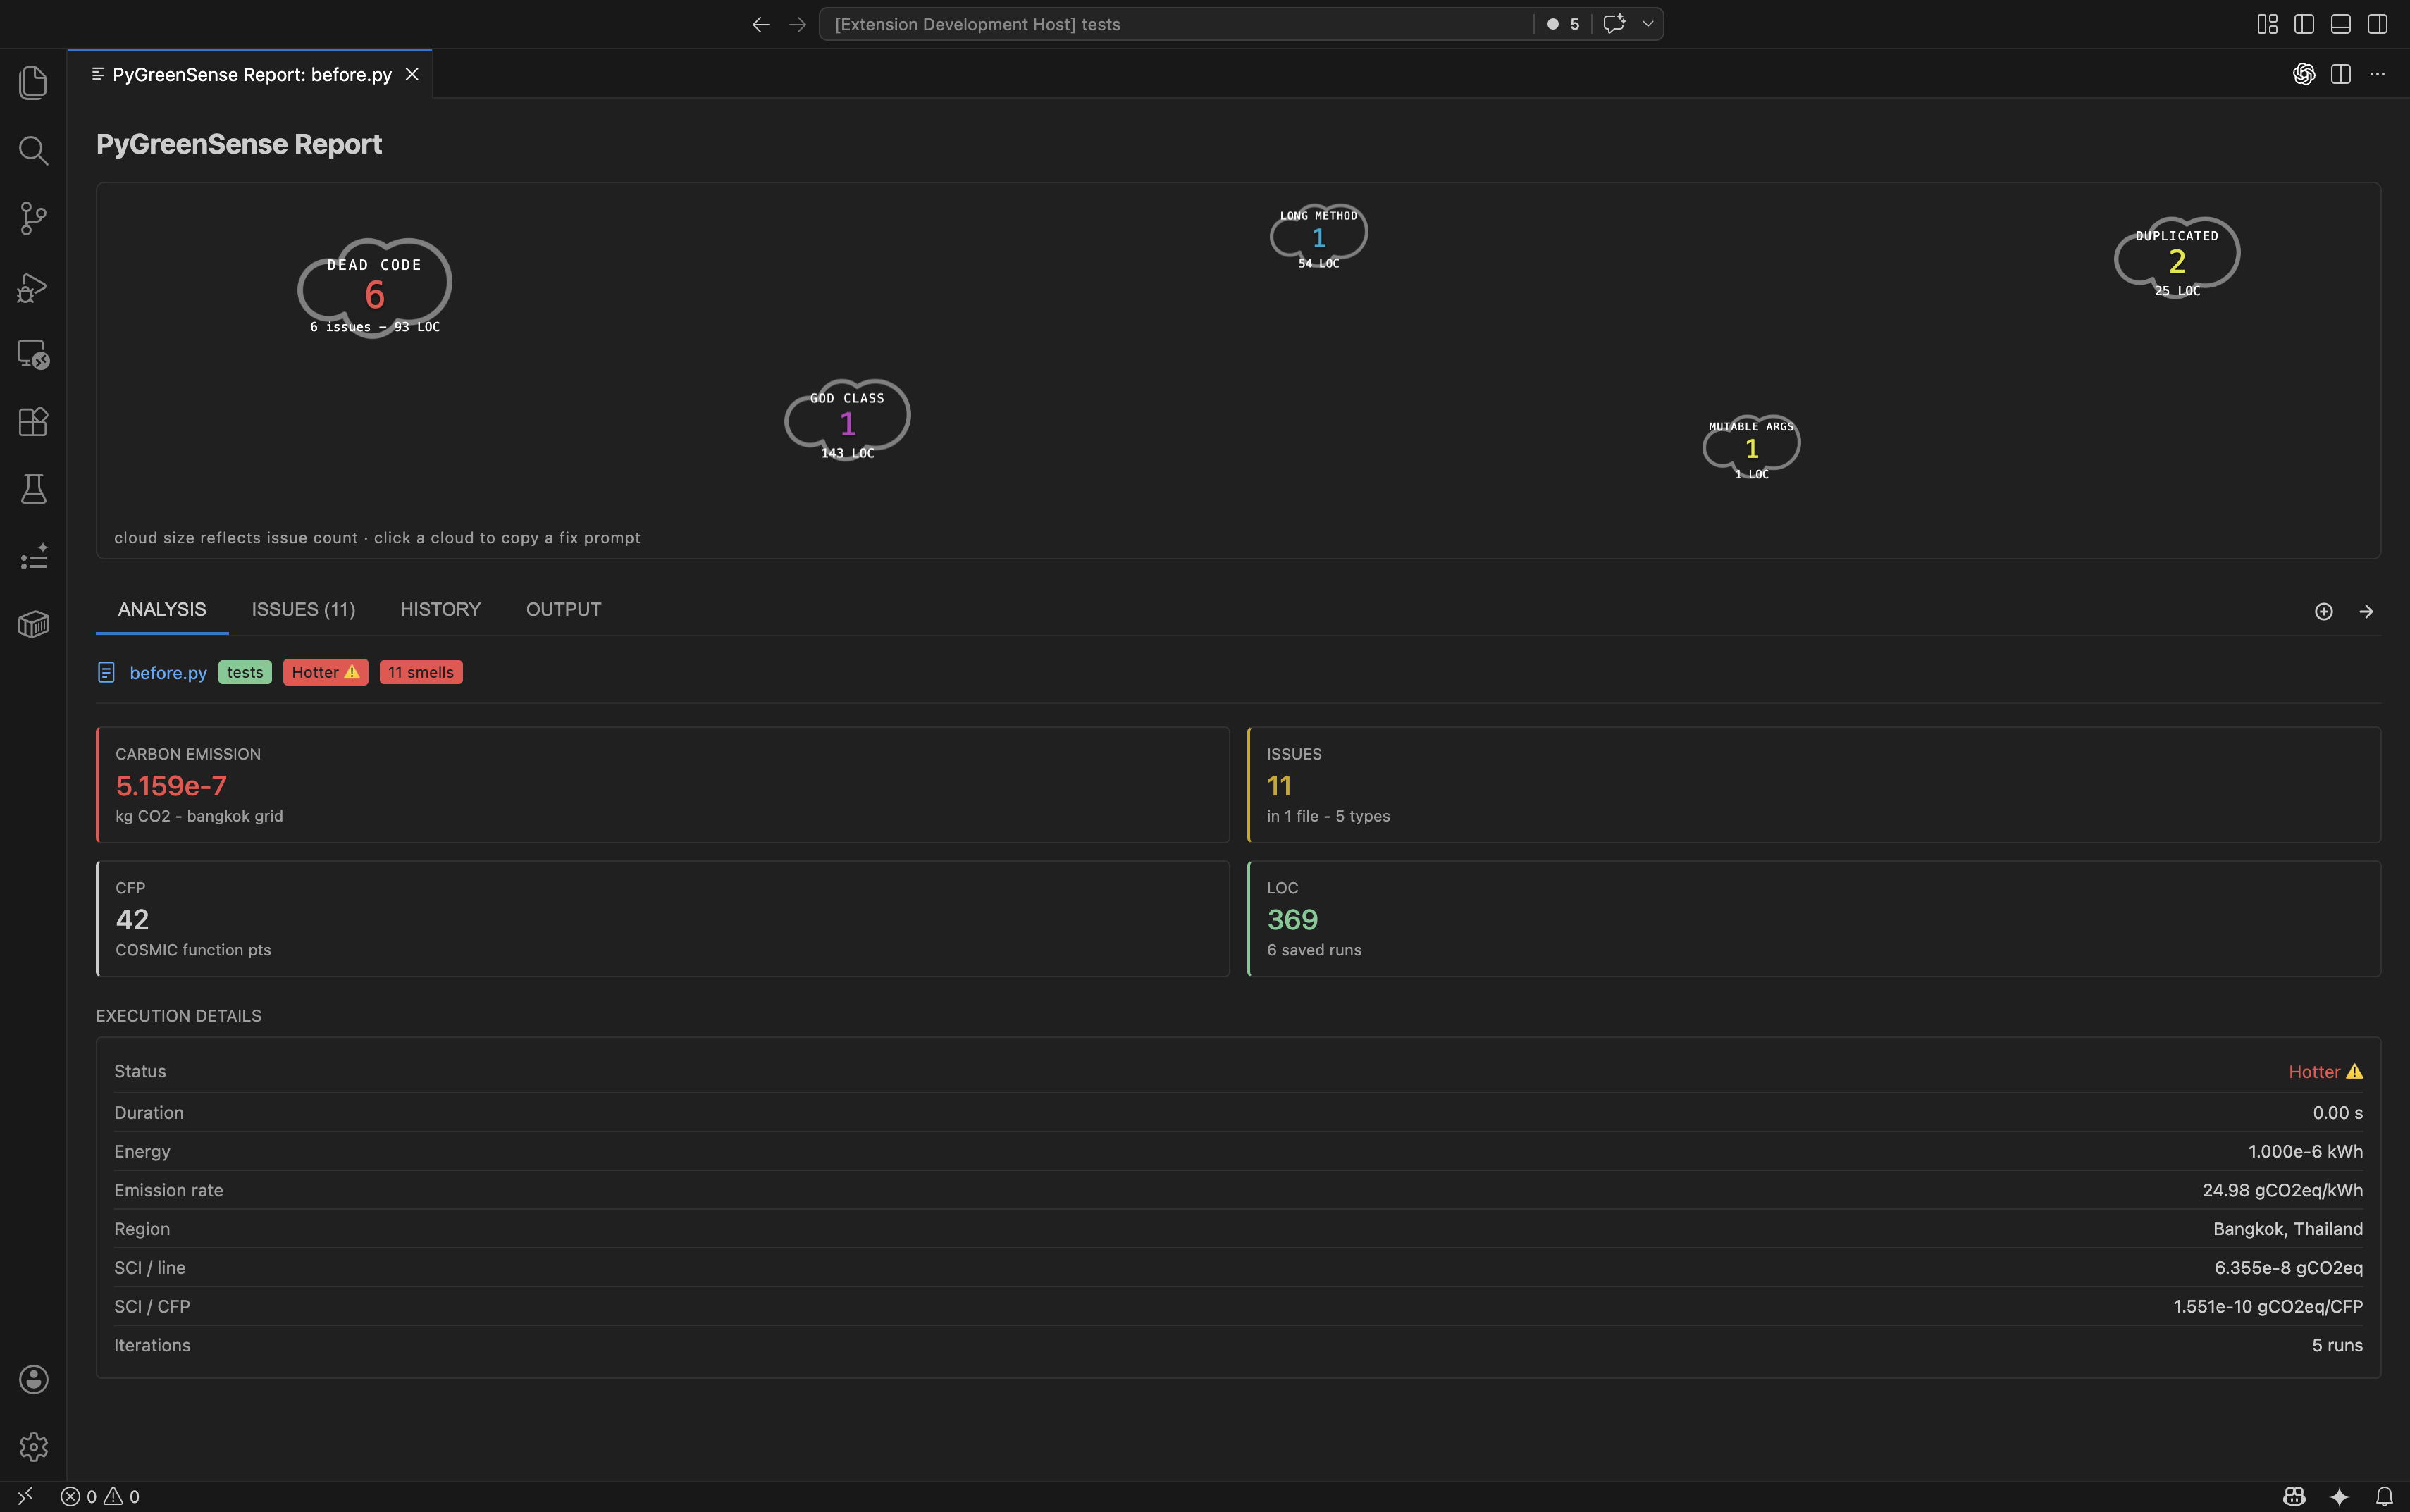
\includegraphics[width=\textwidth]{figures/chap5/webview_analysis_tab.png}
    \captionsetup{name=รูป}
    \caption{หน้าจอแท็บ Analysis ของ Webview Dashboard}
    \label{fig:ch5_webview_analysis}
\end{figure}

\begin{figure}[H]
    \centering
    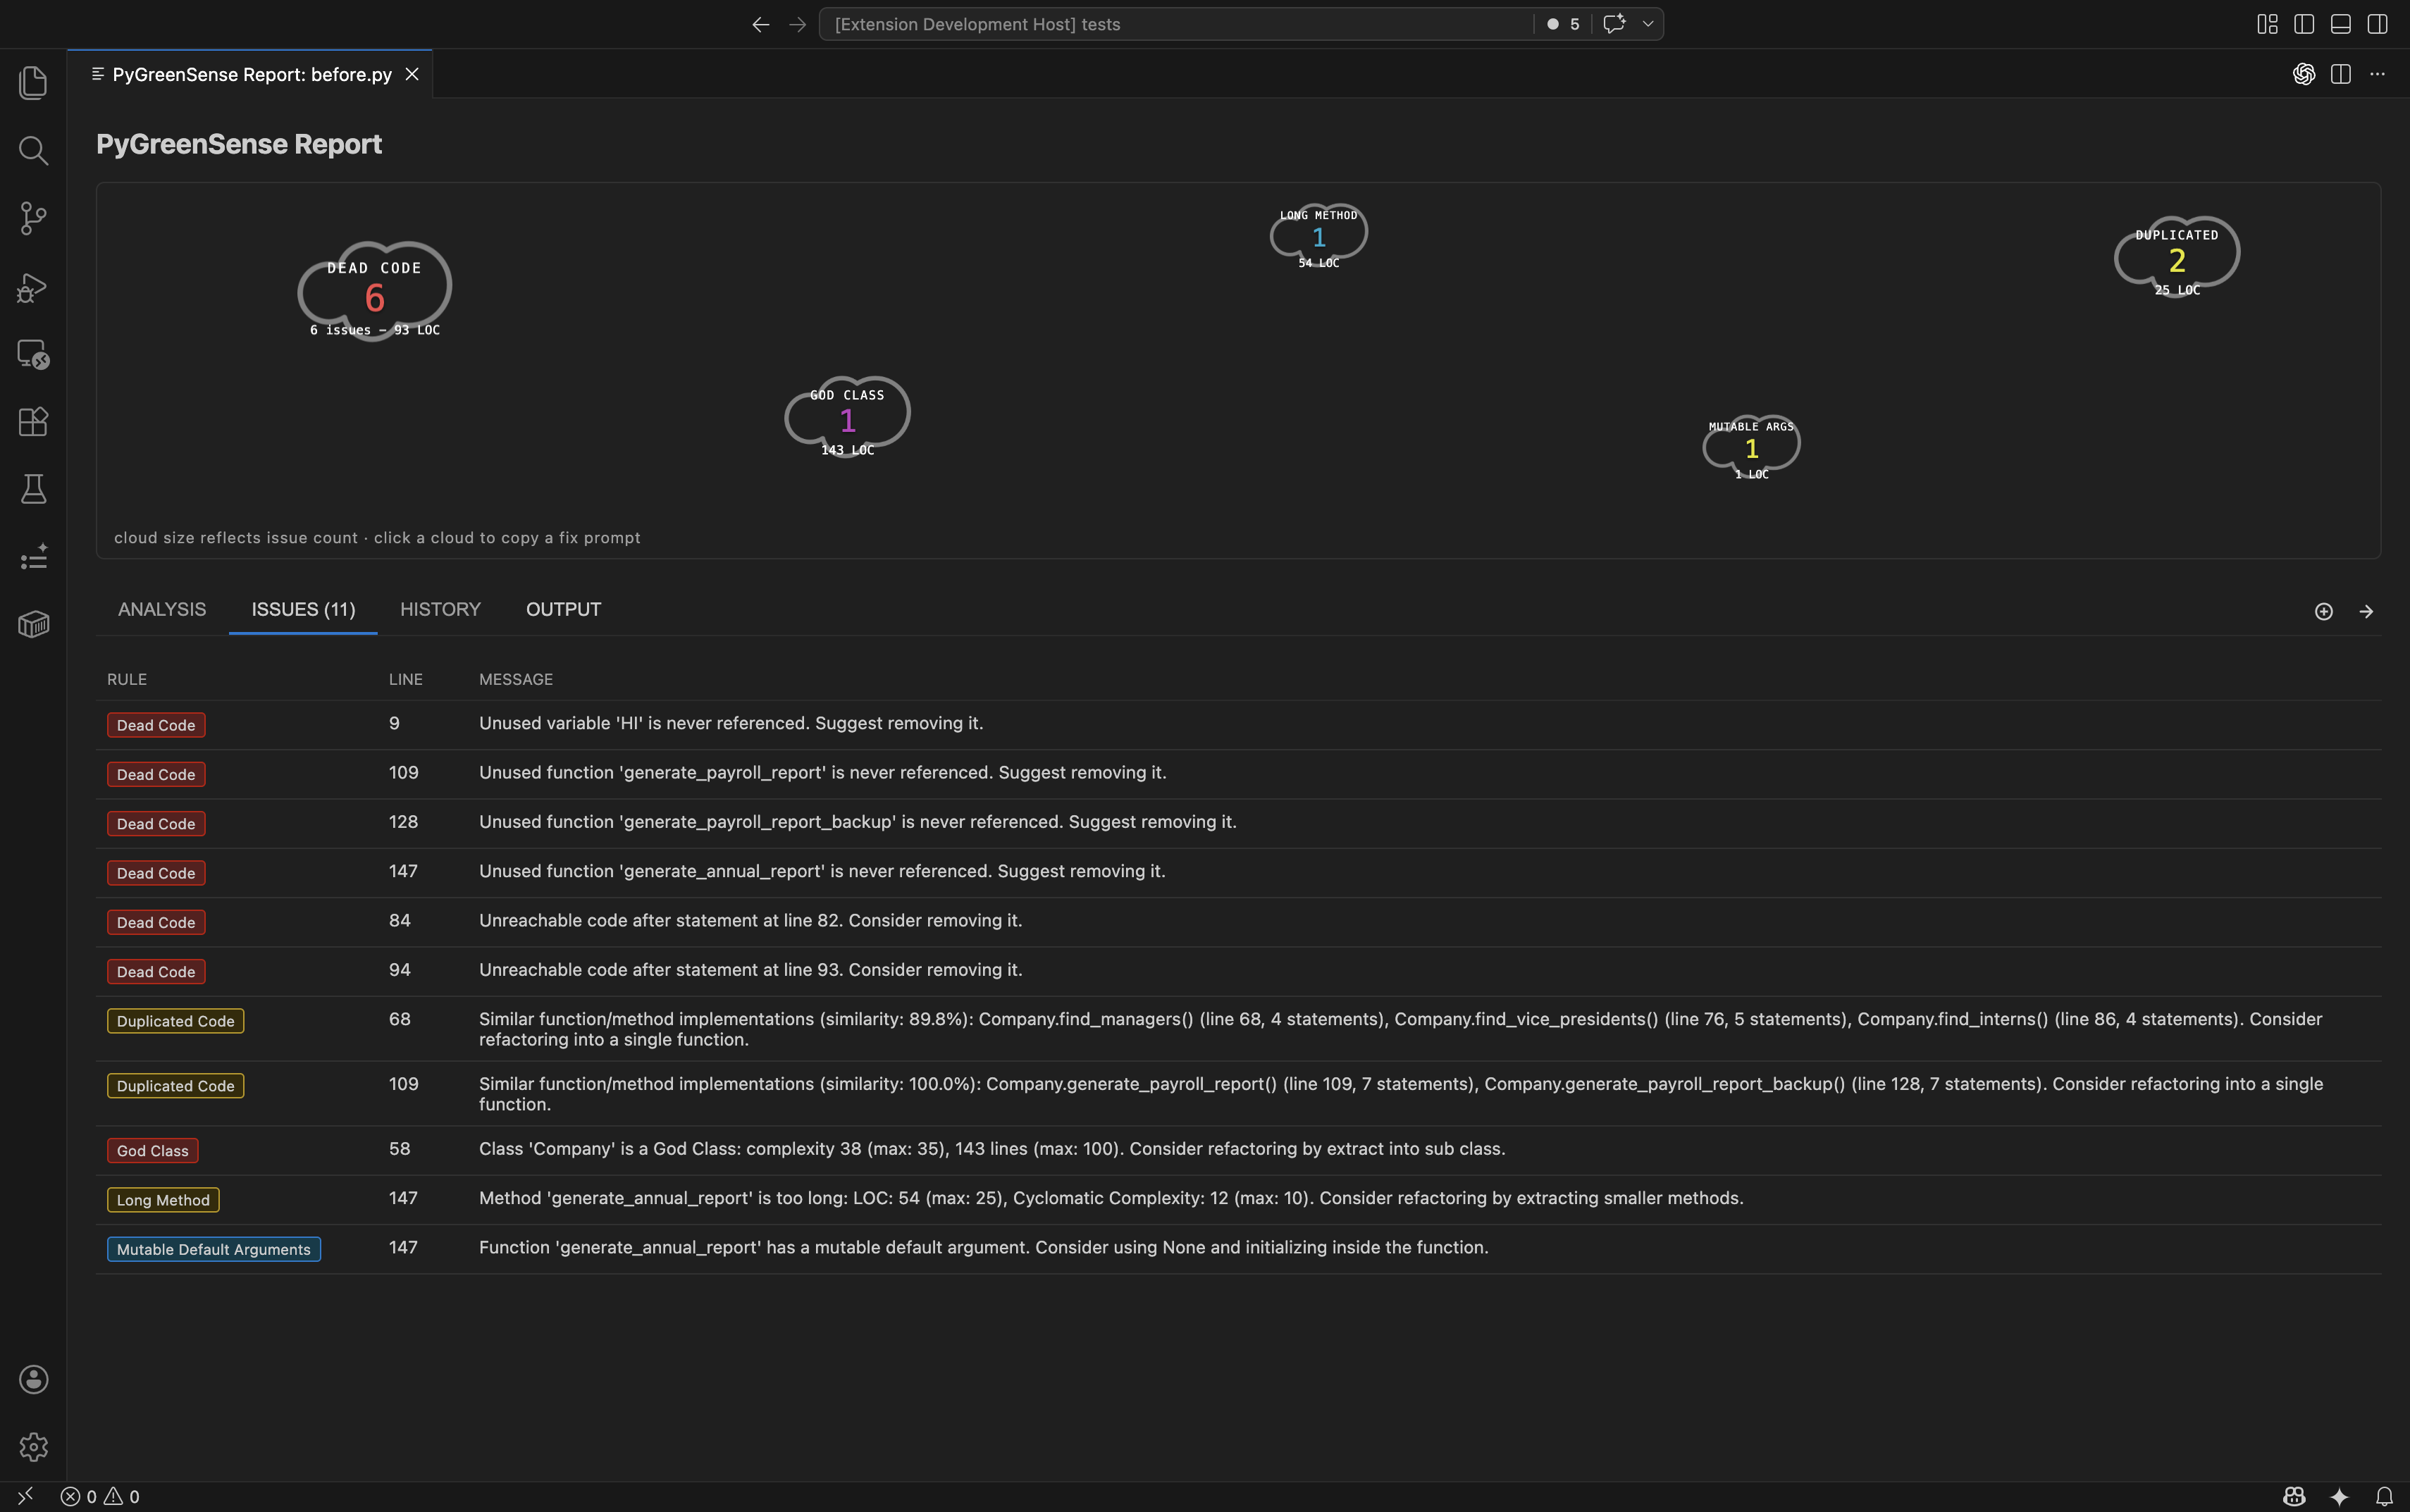
\includegraphics[width=\textwidth]{figures/chap5/webview_issues_tab.png}
    \captionsetup{name=รูป}
    \caption{หน้าจอแท็บ Issues ของ Webview Dashboard}
    \label{fig:ch5_webview_issues}
\end{figure}

\begin{figure}[H]
    \centering
    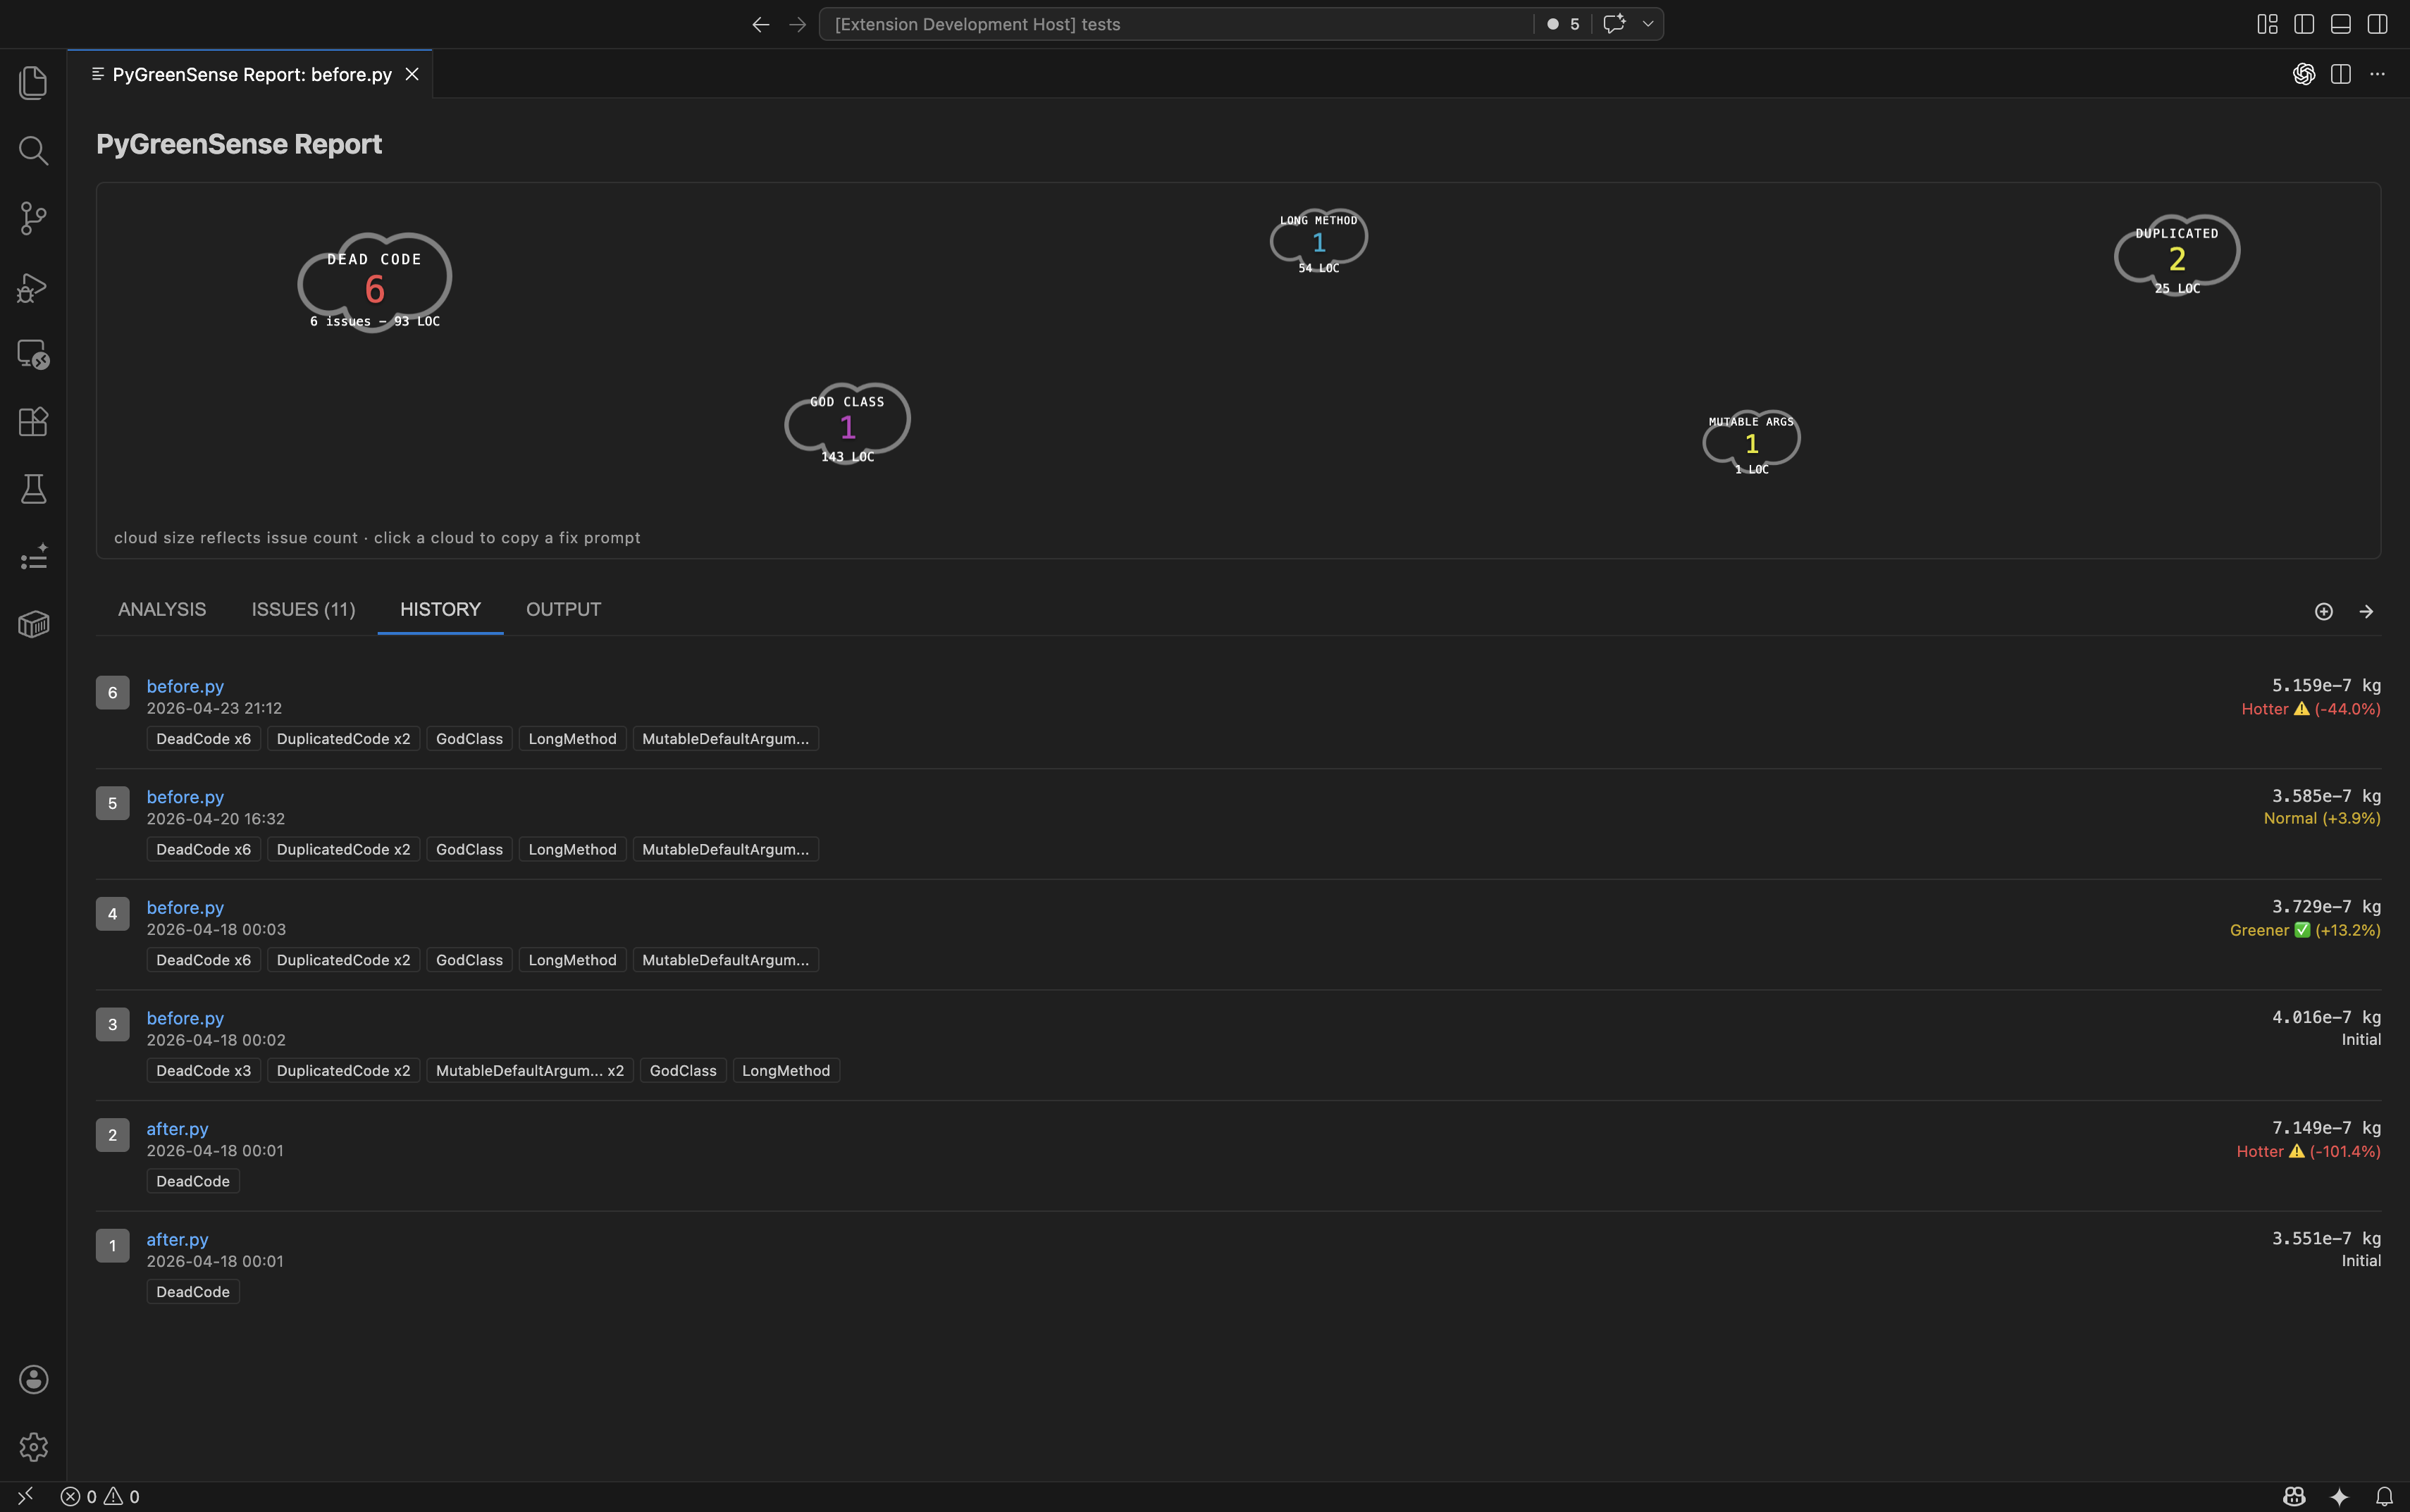
\includegraphics[width=\textwidth]{figures/chap5/webview_history_tab.png}
    \captionsetup{name=รูป}
    \caption{หน้าจอแท็บ History ของ Webview Dashboard}
    \label{fig:ch5_webview_history}
\end{figure}

\begin{figure}[H]
    \centering
    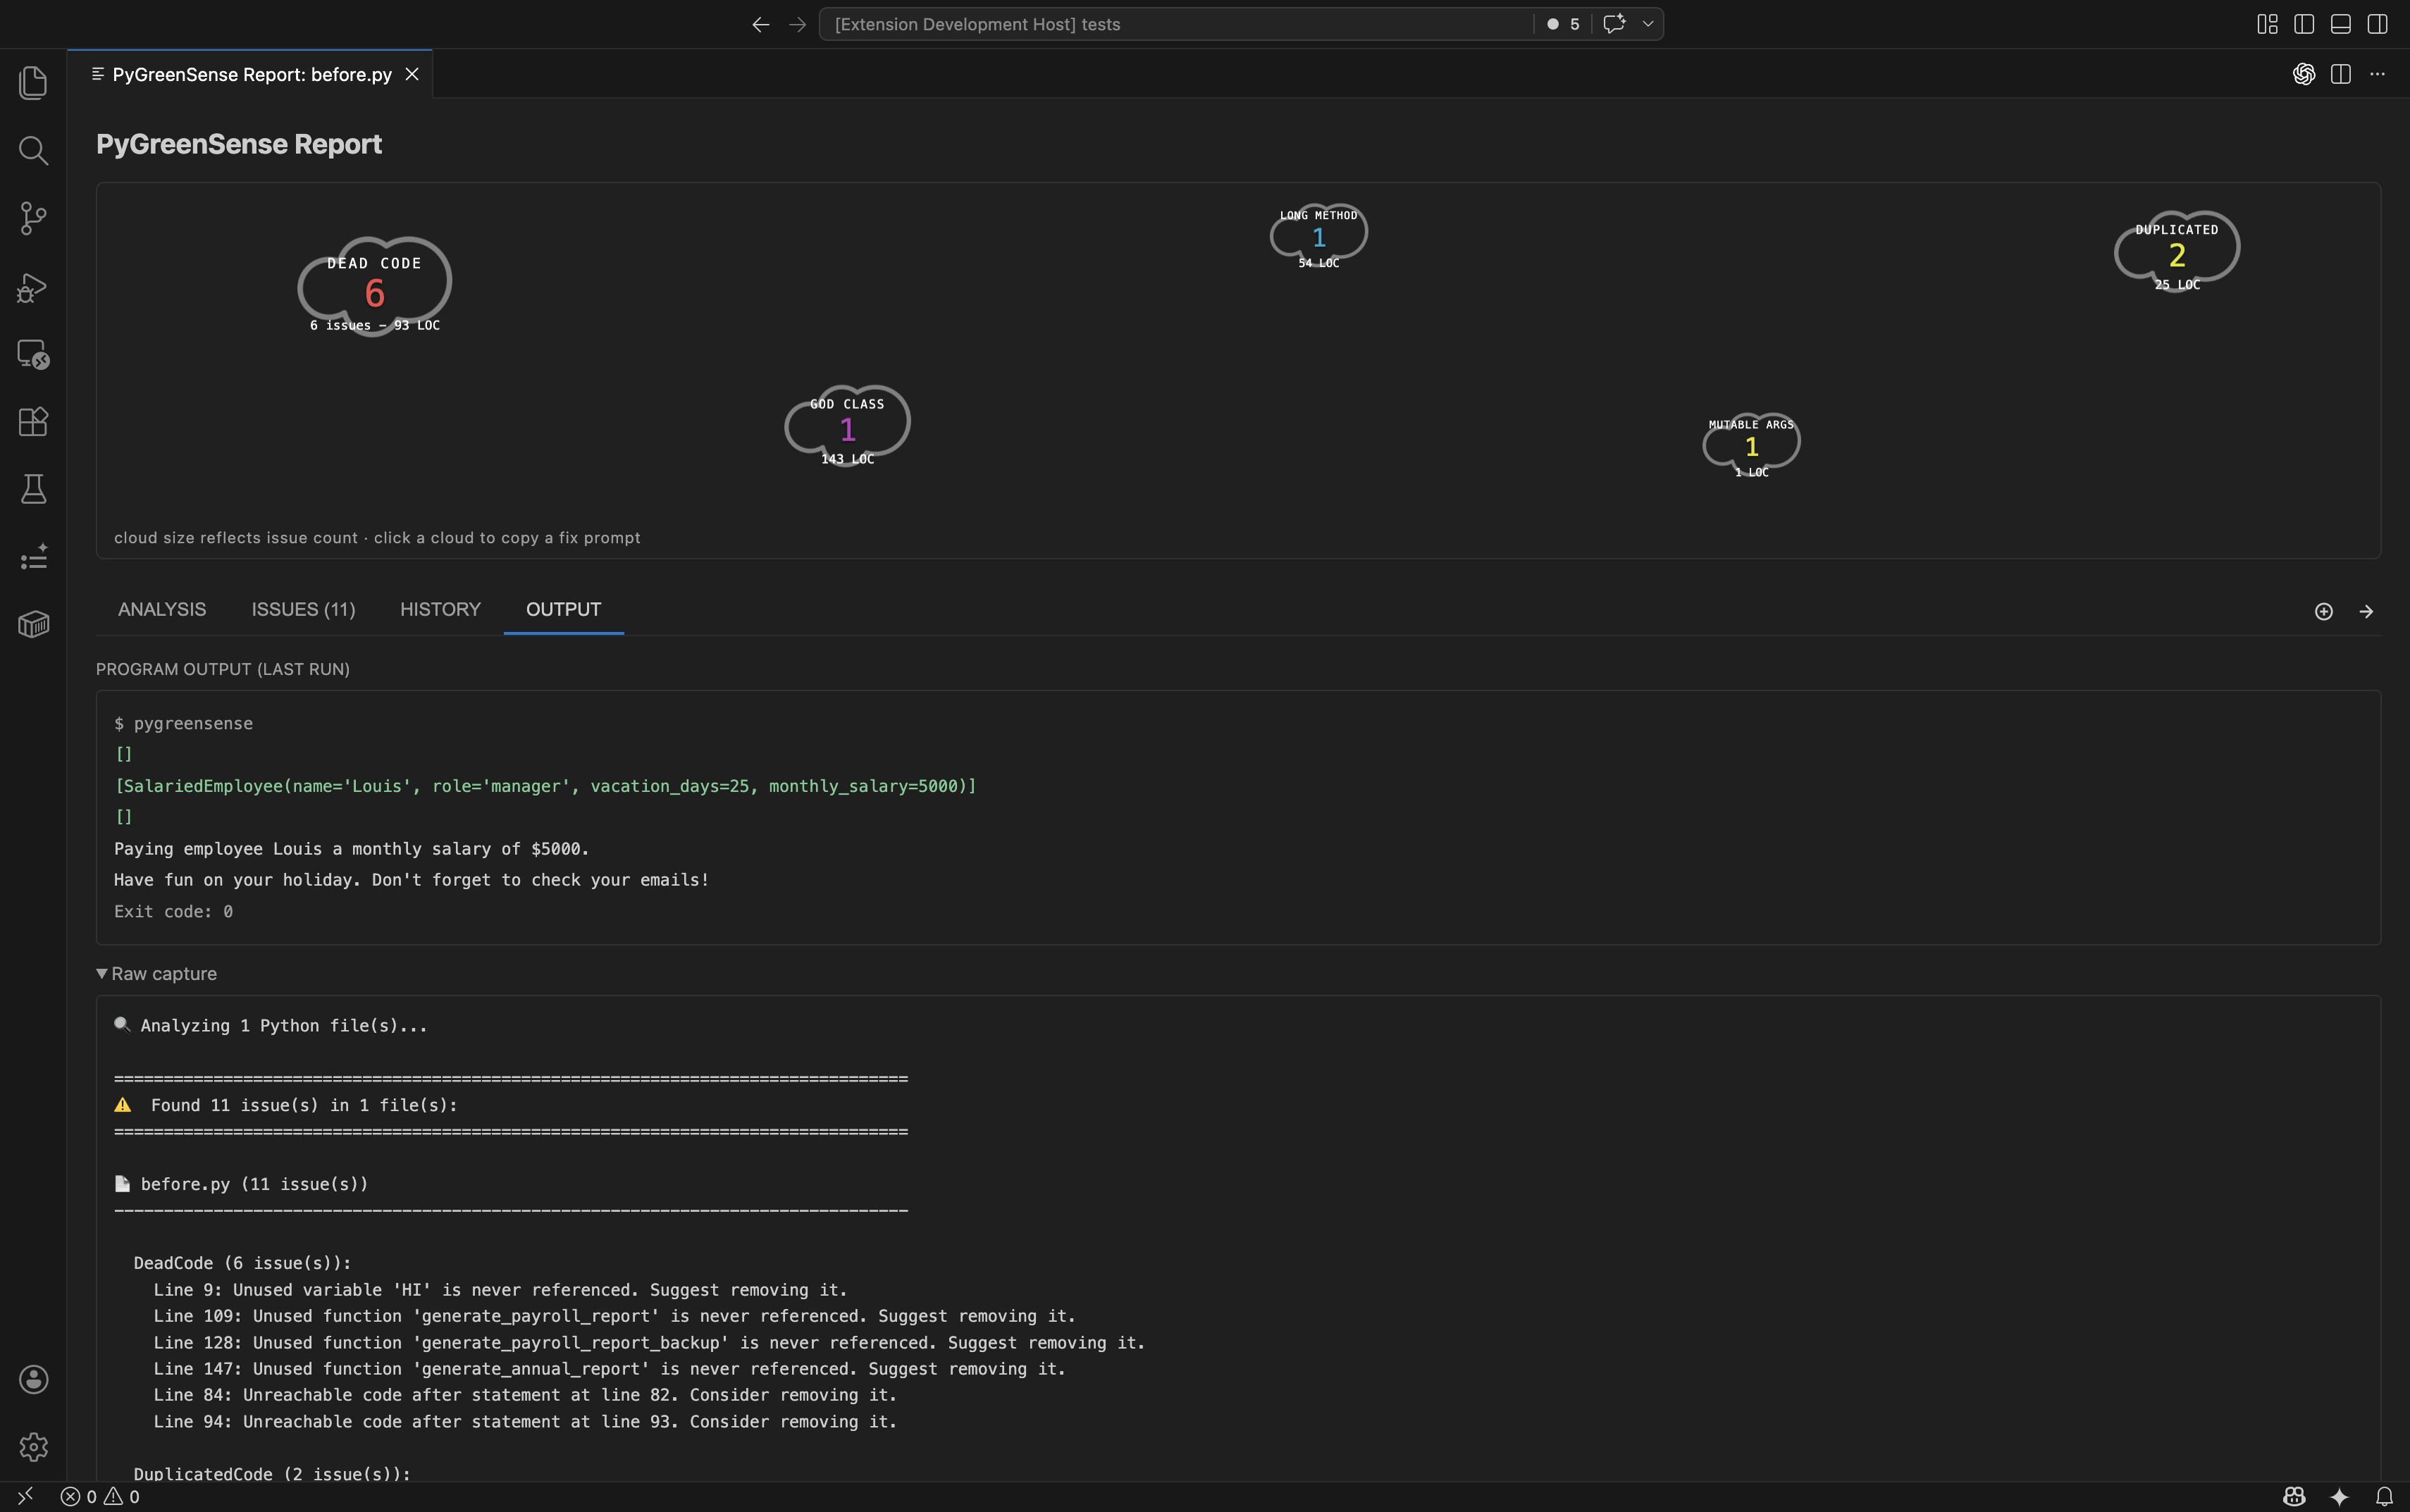
\includegraphics[width=\textwidth]{figures/chap5/webview_output_tab.png}
    \captionsetup{name=รูป}
    \caption{หน้าจอแท็บ Output ของ Webview Dashboard}
    \label{fig:ch5_webview_output}
\end{figure}

\subsection{การประเมินผลมาตรวัดด้านพลังงานและคาร์บอน}

ในระดับการแสดงผล ส่วนขยายรองรับการนำเสนอข้อมูลที่สอดคล้องกับแนวคิดด้าน {\italicfont Software Carbon Intensity (SCI)} และการวัดผลผ่าน {\italicfont CodeCarbon} โดยระบบมีช่องแสดงค่า {\italicfont SCI / line} และ {\italicfont SCI / CFP} อย่างชัดเจน รวมถึงรองรับการแสดงค่า CFP และปริมาณการปล่อยคาร์บอนจากการวิเคราะห์ในแต่ละรอบ

ในเชิงวิธีวิทยา การมีมาตรวัดดังกล่าวช่วยให้ผู้ใช้ไม่ได้เห็นเพียงจำนวน {\italicfont code smell} เท่านั้น แต่ยังเห็นผลกระทบด้านพลังงานและสิ่งแวดล้อมในรูปแบบที่สามารถตีความเชิงเปรียบเทียบได้ ซึ่งสอดคล้องกับแนวคิด {\italicfont SCI per functional unit} ที่กล่าวไว้ในบททฤษฎีที่เกี่ยวข้อง \cite{sciSpecification,codecarbonMethodology,abran2018cosmic}

ดังแสดงในรูป \ref{fig:ch5_webview_analysis} ส่วนของ metric cards และ execution details ถูกออกแบบให้ผู้ใช้เห็นค่าหลัก เช่น carbon emission, CFP, LOC, SCI / line และ SCI / CFP พร้อมกันในหน้ารายงานเดียว ทำให้การตีความผลในเชิงก่อน/หลังการปรับปรุงโค้ดสามารถทำได้สะดวกขึ้น ขณะเดียวกันรูป \ref{fig:ch5_webview_history} และรูป \ref{fig:ch5_webview_output} ช่วยยืนยันว่าระบบรองรับการติดตามผลย้อนหลังและตรวจสอบผลจากการรันล่าสุดได้ภายในรายงานเดียวกัน

\subsection{การประเมินจากการใช้งานจริงของผู้ใช้}

ในส่วนนี้ใช้สำหรับการวัดผลจากการใช้งานจริงของผู้ใช้ เช่น ความพึงพอใจต่อความชัดเจนของ webview ความสะดวกในการใช้งานคำสั่ง ความเข้าใจในค่าพลังงานและคาร์บอน หรือความสามารถของระบบในการช่วยให้ผู้ใช้ตัดสินใจปรับปรุงโค้ดได้ดีขึ้น

อย่างไรก็ตาม ในขอบเขตของฉบับปัจจุบันยังไม่ได้มีการเก็บข้อมูลเชิงปริมาณจากผู้ใช้จริงอย่างเป็นระบบ เช่น แบบสอบถามหรือการทดลองเชิง usability study ดังนั้นบทนี้จึงรายงานผลการประเมินเชิงฟังก์ชันของระบบเป็นหลัก ขณะที่การประเมินความพึงพอใจ ความเข้าใจต่อ metric และผลต่อการตัดสินใจ refactor ของผู้ใช้ จะถูกเสนอเป็นแนวทางการศึกษาต่อยอดในอนาคต

\subsection{การวิเคราะห์ผลในระดับ Extension}

ผลการประเมินในระดับส่วนขยายสะท้อนให้เห็นว่า {\italicfont PyGreenSense Extension} สามารถนำข้อมูลที่ได้จากไลบรารีมาแปลงเป็นรายงานที่มีความเป็นมิตรต่อผู้ใช้และเหมาะกับการใช้งานในสภาพแวดล้อมการพัฒนาจริง โดยเฉพาะการรวมข้อมูลด้าน {\italicfont code smell}, {\italicfont carbon emission}, CFP และประวัติการวิเคราะห์ไว้ในหน้ารายงานเดียว ทำให้ผู้ใช้สามารถมองเห็นทั้งภาพรวมและรายละเอียดของปัญหาได้พร้อมกัน

% -----------------------------------------------------

\section{สรุปผลการประเมิน}

จากการประเมินผลทั้งในระดับไลบรารีและส่วนขยาย VS Code สามารถสรุปได้ว่า {\italicfont PyGreenSense} มีศักยภาพในการทำหน้าที่เป็นเครื่องมือสำหรับตรวจจับ {\italicfont Green Code Smell} ในภาษา Python และสนับสนุนการประเมินผลกระทบด้านพลังงานและคาร์บอนใน {\italicfont workflow} ของนักพัฒนาได้อย่างเป็นรูปธรรม โดยในระดับไลบรารี ระบบสามารถเปรียบเทียบกับเครื่องมืออ้างอิงในอุตสาหกรรมได้ ขณะที่ในระดับ Extension ระบบสามารถนำเสนอผลลัพธ์ผ่าน {\italicfont Webview Dashboard} พร้อมข้อมูลประวัติและมาตรวัดเชิงพลังงานที่เกี่ยวข้องได้อย่างครบถ้วน

อย่างไรก็ตาม หากต้องการให้การประเมินผลมีความสมบูรณ์ยิ่งขึ้นในฉบับสุดท้าย ควรเพิ่มเติมตารางผลการทดลองจริง ค่าความแม่นยำหรือความสอดคล้องเชิงปริมาณของแต่ละ {\italicfont rule} ตัวอย่างผลการเปรียบเทียบก่อนและหลังการปรับปรุงโค้ด และผลจากการใช้งานจริงของผู้ใช้ เพื่อให้การอภิปรายผลมีความชัดเจนและตรวจสอบย้อนกลับได้มากขึ้น

    \clearpage

    \chapter{สรุปและข้อเสนอแนะ}
\label{Ch:Conclusion}

บทนี้นำเสนอผลสรุปของโครงงาน \textit{PyGreenSense} ซึ่งเป็นระบบตรวจจับ Green Code Smell สำหรับภาษา Python ร่วมกับส่วนขยาย Visual Studio Code โดยสรุปผลจากการพัฒนาและการประเมินระบบในบทก่อนหน้า รวมถึงอธิบายข้อจำกัดที่พบระหว่างการดำเนินงาน และเสนอแนวทางสำหรับการพัฒนาต่อยอดในอนาคต

% -----------------------------------------------------

\section{สรุปผลการดำเนินโครงงาน}

โครงงานนี้มีวัตถุประสงค์เพื่อพัฒนาเครื่องมือที่ช่วยให้ผู้พัฒนาโปรแกรมสามารถมองเห็นปัญหาเชิงโครงสร้างของโค้ดที่อาจส่งผลต่อประสิทธิภาพและความยั่งยืนของซอฟต์แวร์ โดยเน้นการตรวจจับ \textit{Green Code Smell} ในภาษา Python และนำเสนอผลลัพธ์ผ่านส่วนขยาย Visual Studio Code เพื่อให้สามารถใช้งานได้ในสภาพแวดล้อมการพัฒนาจริง

ผลลัพธ์หลักของโครงงานคือการพัฒนาไลบรารี \textit{PyGreenSense} ที่สามารถวิเคราะห์ซอร์สโค้ดภาษา Python ด้วยแนวทาง \textit{AST-based static analysis} และตรวจจับ Code Smell ที่เกี่ยวข้องกับคุณภาพของโค้ด ได้แก่ Dead Code, Long Method, God Class, Duplicated Code และ Mutable Default Arguments นอกจากนี้ ระบบยังมีการพัฒนาโมดูลสำหรับจัดเก็บประวัติการวิเคราะห์ในรูปแบบไฟล์ JSON เพื่อรองรับการเปรียบเทียบผลก่อนและหลังการปรับปรุงโค้ด

ในเชิงแนวคิด โครงงานนี้ช่วยให้เห็นภาพของการพัฒนาโค้ดที่มีแนวโน้มเป็นมิตรต่อสิ่งแวดล้อมมากขึ้น หรือ \textit{greener code} โดยไม่ได้พิจารณาเฉพาะความถูกต้องของโปรแกรมเท่านั้น แต่ยังพยายามเชื่อมโยงคุณภาพของโค้ดเข้ากับประเด็นด้านพลังงาน คาร์บอน และความยั่งยืนของซอฟต์แวร์ การพัฒนาดังกล่าวช่วยสะท้อนให้เห็นว่า Code Smell บางประเภทอาจไม่ได้เป็นเพียงปัญหาด้านการอ่านหรือการบำรุงรักษาโค้ด แต่ยังอาจเกี่ยวข้องกับต้นทุนในการประมวลผลและการใช้ทรัพยากรของซอฟต์แวร์ด้วย

อีกประเด็นสำคัญที่โครงงานนี้แสดงให้เห็นคือ เครื่องมือวิเคราะห์โค้ดในปัจจุบันจำนวนมากยังมีข้อจำกัดในการเชื่อมโยงผลการตรวจจับ Code Smell กับผลกระทบด้านพลังงานหรือคาร์บอนโดยตรง เครื่องมือทั่วไปมักเน้นการตรวจจับปัญหาด้านคุณภาพโค้ด เช่น dead code, duplicated code หรือ complexity เป็นหลัก แต่ยังไม่ได้อธิบายว่าปัญหาเหล่านี้ส่งผลต่อมิติด้าน Green Software Engineering อย่างไร ดังนั้น \textit{PyGreenSense} จึงเป็นแนวทางหนึ่งในการทดลองเชื่อมช่องว่างระหว่างการวิเคราะห์คุณภาพโค้ดและการประเมินผลกระทบด้านความยั่งยืนของซอฟต์แวร์

% -----------------------------------------------------

\section{สรุปผลการพัฒนาระบบ}

จากการพัฒนา ระบบ \textit{PyGreenSense} ประกอบด้วยองค์ประกอบหลัก ได้แก่ AST Parser, ชุดกฎสำหรับตรวจจับ Green Code Smell, Metric and Analysis Module, VS Code Extension Module และ Reporting Module โดยแต่ละส่วนทำงานร่วมกันเพื่อให้สามารถวิเคราะห์โค้ด ตรวจจับปัญหา จัดเก็บผลลัพธ์ และแสดงผลให้ผู้ใช้เข้าใจได้ง่ายขึ้น

ในส่วนของไลบรารีตรวจจับ ระบบสามารถใช้ AST ของภาษา Python เพื่อวิเคราะห์โครงสร้างของโปรแกรมในระดับฟังก์ชัน คลาส ตัวแปร และคำสั่งต่าง ๆ ได้อย่างเป็นระบบ กฎการตรวจจับที่พัฒนาขึ้นสามารถระบุปัญหาที่พบได้ เช่น ฟังก์ชันที่ยาวเกินไป คลาสที่มีความรับผิดชอบมากเกินไป โค้ดที่ซ้ำกัน โค้ดที่ไม่ได้ใช้งาน และการใช้ค่าเริ่มต้นของพารามิเตอร์ที่เป็น mutable object

ในส่วนของมาตรวัด ระบบได้เพิ่มแนวคิดการคำนวณ \textit{Cosmic Function Points (CFP)} เพื่อประมาณขนาดเชิงฟังก์ชันของซอฟต์แวร์จากซอร์สโค้ด และนำแนวคิด \textit{Software Carbon Intensity (SCI)} มาประยุกต์ใช้ในรูปแบบ SCI per CFP เพื่อพิจารณาปริมาณคาร์บอนต่อหน่วยงานที่ซอฟต์แวร์ทำจริง นอกจากนี้ ระบบยังมีตรรกะสำหรับเปรียบเทียบผลก่อนและหลังการปรับปรุงโค้ด เช่น Impact Logic และ Rule-based Estimated Saving เพื่อใช้วิเคราะห์แนวโน้มผลกระทบของการลด Code Smell

ในส่วนของ VS Code Extension ระบบถูกออกแบบให้ช่วยให้ผู้ใช้สามารถเรียกใช้งานการวิเคราะห์ได้สะดวกขึ้นจากภายในเครื่องมือพัฒนาโค้ด โดยมีแนวคิดในการจัดการ environment ของไลบรารี การเรียกใช้งานระบบตรวจจับ และการแสดงผลลัพธ์ในรูปแบบที่ผู้ใช้สามารถนำไปใช้ประกอบการตัดสินใจปรับปรุงโค้ดได้

% -----------------------------------------------------

\section{สรุปผลการประเมิน}

ผลการประเมินแสดงให้เห็นว่า \textit{PyGreenSense} สามารถตรวจจับ Green Code Smell ตามกฎที่กำหนดไว้ได้ และสามารถนำข้อมูลผลลัพธ์ไปใช้ประกอบการวิเคราะห์ก่อนและหลังการปรับปรุงโค้ดได้ในระดับหนึ่ง โดยเฉพาะการเปรียบเทียบจำนวน Code Smell ที่ลดลงหลังการ refactor และการจัดเก็บข้อมูลใน History Log เพื่อใช้ติดตามผลลัพธ์ในระยะยาว

อย่างไรก็ตาม ผลการประเมินยังสะท้อนข้อจำกัดสำคัญของการทดลองในปัจจุบัน กล่าวคือ ชุดโค้ดที่ใช้ในการทดสอบยังมีจำนวนและความหลากหลายจำกัด ทำให้ผลลัพธ์ด้านพลังงานและคาร์บอนยังไม่สามารถสรุปได้อย่างครอบคลุมในทุกสถานการณ์ โดยเฉพาะในกรณีที่ source code มีขนาดเล็กหรือมี workload ไม่มากพอ ค่าพลังงานที่วัดได้อาจมีความผันผวนจากสภาพแวดล้อมของเครื่องที่ใช้ทดสอบ และอาจทำให้การตีความผลกระทบของการ refactor ต่อการลดคาร์บอนยังไม่ชัดเจน

นอกจากนี้ ผลกระทบของ Code Smell แต่ละประเภทต่อการใช้พลังงานยังมีข้อมูลเชิงประจักษ์ค่อนข้างน้อย แม้ระบบจะสามารถตรวจจับและลดจำนวน Code Smell ได้ แต่ยังไม่สามารถสรุปได้แน่ชัดว่า Code Smell แต่ละประเภทส่งผลต่อพลังงานหรือคาร์บอนมากน้อยเพียงใดในทุกกรณี ตัวอย่างเช่น การลด Dead Code หรือ Long Method อาจช่วยให้โค้ดอ่านง่ายและบำรุงรักษาได้ดีขึ้นอย่างชัดเจน แต่ผลด้านพลังงานอาจขึ้นอยู่กับลักษณะการทำงานจริงของโปรแกรม ขนาดข้อมูลที่ใช้ทดสอบ และจำนวนครั้งที่โค้ดส่วนนั้นถูกเรียกใช้งาน

ดังนั้น ข้อสรุปสำคัญจากการประเมินคือ การลด Code Smell สามารถช่วยปรับปรุงคุณภาพของโค้ดและทำให้แนวทางการพัฒนาโค้ดมีความเป็นระบบมากขึ้น แต่ผลกระทบด้านพลังงานและคาร์บอนยังควรถูกตีความในฐานะผลลัพธ์เชิงประมาณการหรือแนวโน้มเบื้องต้น มากกว่าการยืนยันผลเชิงสรุปในทุกสถานการณ์

% -----------------------------------------------------

\section{ข้อจำกัดของโครงงาน}

แม้ว่าโครงงานนี้จะสามารถพัฒนาเครื่องมือตรวจจับ Green Code Smell และเชื่อมโยงกับมาตรวัดด้านคาร์บอนได้ในระดับหนึ่ง แต่ยังมีข้อจำกัดที่ควรพิจารณา ดังนี้

\begin{itemize}
    \item {\boldfont ข้อจำกัดด้านชุดโค้ดทดสอบและ Bias ของข้อมูล}
    ชุดโค้ดที่ใช้ยังมีขนาดและความหลากหลายจำกัด และบางส่วนเป็น {\italicfont mock code} ที่มีลักษณะเรียบง่าย เช่น {\italicfont dead code} หรือ {\italicfont mutable default argument} แบบตรงไปตรงมา รวมถึงการ refactor ที่ไม่สม่ำเสมอ ทำให้ไม่สามารถสะท้อนสถานการณ์จริงได้ครบถ้วน และอาจเกิด {\italicfont bias} ที่ส่งผลให้ผลลัพธ์ยังไม่สามารถ {\italicfont generalize} ไปยังระบบจริงได้

    \item {\boldfont ข้อจำกัดด้านผลกระทบของ Code Smell แต่ละประเภท}
    ข้อมูลเชิงประจักษ์เกี่ยวกับผลกระทบของ Code Smell แต่ละประเภทต่อการใช้พลังงานยังมีไม่มากพอ ทำให้การวิเคราะห์ผลกระทบของแต่ละ smell ยังเป็นการประมาณจากข้อมูลที่ระบบตรวจพบ เช่น จำนวนบรรทัดที่ถูกลดลง จำนวน smell ที่ลดลง หรือค่าคาร์บอนที่เปลี่ยนแปลงหลังการทดสอบ

    \item {\boldfont ข้อจำกัดด้านการวัดพลังงานและคาร์บอน}
    ผลการวัดพลังงานและคาร์บอนอาจได้รับผลกระทบจากสภาพแวดล้อมของเครื่องที่ใช้ทดสอบ เช่น background process, hardware, operating system และลักษณะการรันโปรแกรมในแต่ละครั้ง ทำให้ค่าที่ได้อาจมีความผันผวน

    \item {\boldfont ข้อจำกัดด้านขอบเขตของ Static Analysis}
    ระบบใช้การวิเคราะห์จากโครงสร้าง AST เป็นหลัก จึงสามารถตรวจจับปัญหาเชิงโครงสร้างของโค้ดได้ดีในระดับหนึ่ง แต่ยังมีข้อจำกัดในการวิเคราะห์พฤติกรรมที่เกิดขึ้นจริงระหว่าง runtime เช่น input ที่เปลี่ยนแปลงตามสถานการณ์ หรือโค้ดที่ถูกเรียกใช้งานผ่าน dynamic behavior

    \item {\boldfont ข้อจำกัดด้านการใช้งานของผู้เริ่มต้น}
    แม้ระบบจะช่วยแสดงผล Code Smell ได้ แต่การอธิบายผลลัพธ์และการแนะนำวิธีแก้อาจยังเข้าใจยาก และอาศัยความเข้าใจค่อนข้างสูงสำหรับผู้เริ่มต้นเขียนโค้ด

    \item {\boldfont ข้อจำกัดของ SCI (Software Carbon Intensity) ในบางกรณี}
    แม้จะลด LOC, CFP หรือจำนวน {\italicfont code smell} ลงอย่างมาก แต่ค่าคาร์บอนหรือ SCI อาจไม่ได้ลดลงตาม หรืออาจเพิ่มขึ้น เนื่องจาก SCI ขึ้นอยู่กับพฤติกรรม {\italicfont runtime} และปัจจัยแวดล้อมอื่น ๆ ทำให้ไม่สามารถใช้เป็นตัวชี้วัดผลของการ refactor ได้โดยตรงในทุกกรณี
\end{itemize}

% -----------------------------------------------------

\section{ข้อเสนอแนะสำหรับการพัฒนาต่อ}

จากผลการดำเนินงานและข้อจำกัดที่พบ สามารถเสนอแนวทางพัฒนาต่อในอนาคตได้ดังนี้

\begin{itemize}
    \item {\boldfont การปรับปรุงมาตรฐานและความน่าเชื่อถือของการวัด (Standardization \& Reliability)}
    ควรพัฒนา {\italicfont baseline}, {\italicfont threshold} และ {\italicfont Data Catalog} สำหรับผลกระทบของ Code Smell ต่อพลังงานและคาร์บอน เพื่อให้สามารถเปรียบเทียบผลได้อย่างเป็นมาตรฐานและลดความคลาดเคลื่อนของการวิเคราะห์

    \item {\boldfont การพัฒนา Refactoring Suggestion และ Editor Integration}
    ควรพัฒนาระบบแนะนำแนวทางแก้ไข Code Smell และเชื่อมต่อกับ {\italicfont code editor} เช่น VS Code Extension เพื่อช่วยให้ผู้ใช้สามารถปรับปรุงโค้ดได้แบบ {\italicfont real-time} และใช้งานได้สะดวกยิ่งขึ้น

    \item {\boldfont การขยายกฎการตรวจจับ Code Smell}
    ควรเพิ่มจำนวนและความหลากหลายของ {\italicfont code smell rules} รวมถึงรองรับ {\italicfont pattern} ที่พบในโปรเจกต์จริงมากขึ้น เพื่อให้ครอบคลุมปัญหาด้านคุณภาพโค้ดได้ดียิ่งขึ้น

    \item {\boldfont การพัฒนาการแสดงผลและ Visualization (Gamification)}
    ควรออกแบบการแสดงผลให้น่าสนใจมากขึ้น เช่น การใช้ {\italicfont score}, {\italicfont badge} หรือระดับ ({\italicfont level}) เพื่อช่วยให้ผู้ใช้เข้าใจผลลัพธ์ได้ง่ายและสร้างแรงจูงใจในการเขียนโค้ดที่มีประสิทธิภาพมากขึ้น

    \item {\boldfont การเพิ่มประสิทธิภาพสำหรับโปรเจกต์ขนาดใหญ่ (Scalability)}
    ควรปรับปรุงประสิทธิภาพของระบบให้สามารถวิเคราะห์ {\italicfont source code} ขนาดใหญ่ได้รวดเร็วและมีประสิทธิภาพมากขึ้น รวมถึงรองรับโครงสร้างโปรเจกต์ที่ซับซ้อน

    \item {\boldfont การเพิ่มชุดทดสอบและข้อมูลจากการใช้งานจริง}
    ควรรวบรวม {\italicfont source code} และ {\italicfont log} จากการใช้งานจริงเพื่อนำมาวิเคราะห์และลด {\italicfont bias} ของ {\italicfont mock data} รวมถึงช่วยให้ผลลัพธ์มีความสมจริงและน่าเชื่อถือมากขึ้น
\end{itemize}

% -----------------------------------------------------

\section{สรุปภาพรวม}

โดยสรุป โครงงาน \textit{PyGreenSense} สามารถพัฒนาเครื่องมือตรวจจับ Green Code Smell สำหรับภาษา Python และแสดงให้เห็นแนวทางเบื้องต้นในการเชื่อมโยงคุณภาพของโค้ดเข้ากับประเด็นด้านพลังงานและคาร์บอนของซอฟต์แวร์ได้สำเร็จ โครงงานนี้ช่วยให้เห็นภาพว่าการพัฒนาโค้ดที่ดีไม่ได้จำกัดอยู่เพียงความถูกต้องหรือความง่ายต่อการบำรุงรักษาเท่านั้น แต่ยังสามารถขยายไปสู่แนวคิดการพัฒนาโค้ดที่คำนึงถึงความยั่งยืนได้ด้วย

อย่างไรก็ตาม ผลลัพธ์ด้านพลังงานและคาร์บอนยังมีข้อจำกัดจากชุดทดสอบและข้อมูลผลกระทบของแต่ละ Code Smell ที่ยังมีจำนวนน้อย ดังนั้นการพัฒนาต่อควรมุ่งเน้นการเก็บข้อมูลเชิงประจักษ์เพิ่มเติม การสร้าง Data Catalog ของผลกระทบ Code Smell ในภาษา Python และการนำข้อมูลจากการใช้งานจริงของ Extension และ Library มาวิเคราะห์ เพื่อให้สามารถพัฒนาเครื่องมือที่ช่วยผู้ใช้เขียนโค้ดได้ดีขึ้น มีประสิทธิภาพมากขึ้น และตระหนักถึงผลกระทบด้านพลังงานของซอฟต์แวร์มากขึ้นในอนาคต

    \clearpage

    % \chapter{ทดสอบ}
\label{Ch:TEST}

\section{ทดสอบ 1}
โชกี้ บทที่\ref{Ch:TEST} {\boldfont ตัวหนา} {\italicfont ตัวเอียง} \underline{วิทยาศาสตร์} \\นางฟ้า IT

Hello Dear

\subsection{ทดสอบย่อย 1}

\section{ทดสอบ 2}
\begin{itemize}
    \item first item
    จิตรกัณฐ์ ดำรงตระกูลวัฒน์
    \item second item
    \item third item
\end{itemize}

\begin{enumerate}
    \item first item
    \item second item
    \item third item
\end{enumerate}

\begin{table}[]
    \centering
    \begin{tabular}{c|c}
         &  \\
         & 
    \end{tabular}
    \caption{Caption}
    \label{tab:placeholder}
\end{table}

\cite{parker2020}

ตัวอย่างการเพิ่มตารางและการอ้างอิงไปยังตาราง \ref{table:example_table}.

\begin{table}[h]
\centering
\begin{tabular}{|c c c|}
\hline
คอลัมน์1 & คอลัมน์2 & คอลัมน์3 \\ 
\hline
A & xx & xx \\ 
\hline
B & yy & yy \\ 
\hline
C & xx & xx  \\
%\hline
E & ZZ & ZZ \\
\hline
\end{tabular}
\captionsetup{justification=centering, name=ตาราง}
\caption{คำบรรยายตาราง}
\label{table:example_table}
\end{table}

ตัวอย่างการอ้างอิงไปยังบทความในเอกสารอ้างอิง \cite{parker2020}. 

วิธีการเพิ่มรูปภาพและอ้างอิงไปยังรูปภาพ \ref{fig:example_figure}

\begin{figure}[h]
    \centering
    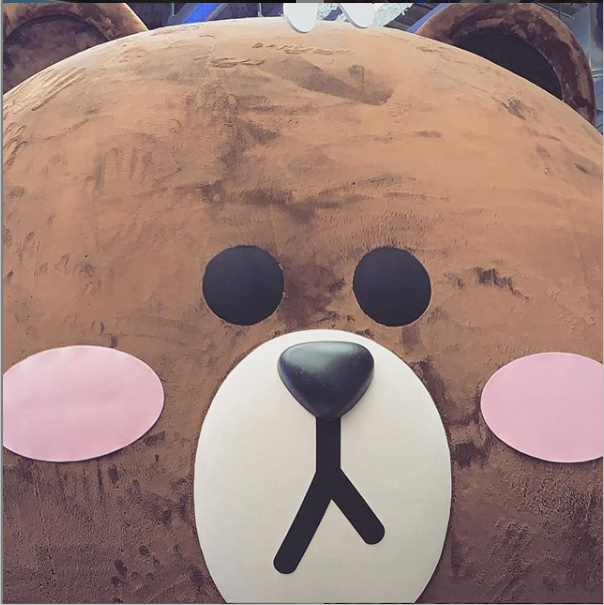
\includegraphics[scale = 0.3]{figures/chap2/Sample101.PNG}
    \captionsetup{name = รูป}
    \caption{คำอธิบายรูปภาพ}
    \label{fig:example_figure}
\end{figure}

วิธีการเพิ่ม{\boldfont สมการ} และ{\italicfont อ้างอิง}ไปยังสมการ \ref{eq:example_equation}.

\begin{equation} 
y = \sqrt{x^2+1}
\label{eq:example_equation}
\end{equation}

\begin{equation}
    x=\frac{a}{b}
    X=\sum_{i=1}^{n} x_1
\end{equation}

\begin{itemize}
    \item AST Parser
    \item ชุดกฎ Green Code Smell
        \begin{itemize}
            \item Long Loop Without Break
            \item Repeated Object Creation
            \item Unnecessary I/O Operations
            \item Inefficient Collection Usage
        \end{itemize}
    \item Metric \& Analysis Module
    \item Reporting Module
\end{itemize}
    % \clearpage

    \bibliographystyle{styles/muict}
    \bibliography{bibliography/reference}
    \clearpage
    % \input{frontmatter/AIstatement.tex}
    % \clearpage
    % \input{appendices/appendixA.tex}
    % \clearpage
    % \input{appendices/appendixB.tex}
    % \clearpage

\end{document}
